\chapter{Proposta de Melhorias de Design para o Mezuro}
\label{chap:proposta}

Este capítulo é dedicado à exposição das propostas de melhorias de apresentação
ou visualização dos repositórios analisados pelo Mezuro. Na primeira seção, são
apresentadas as telas desenhadas pelo aluno com base na experiência com outras
ferramentas de avaliação de código-fonte. E também, outras pequenas evoluções
na disposição dos itens já existentes no Mezuro. A segunda seção trata da
disposição de possíveis técnicas de VS aplicáveis ao Mezuro, bem como um pequeno
exemplo de uso, seguido da apresentação dos resultados de uma pesquisa com as
visualizações criadas neste exemplo de uso.

Inicialmente, foi considerado como uma abordagem ideal a aplicação dessas
técnicas de visualização de software, que era o objetivo do TCC 1. Isso
justifica todo o estudo e levantamento bibliográfico do Capítulo
\ref{chap:visualizacao}. Porém, após todos os desafios apresentados no Capítulo
anterior a este, uma nova aposta de evolução foi levantada e é a descrita no
restante deste capítulo, como segundo conjunto de contribuições.

\section{Proposta de Evolução}

A seguir são dispostas os protótipos das telas idealizadas pelo aluno. São
pequenas modificações na disposições de elementos já presentes na página de
\textit{view} dos repositórios adicionados no Mezuro (vide Figura
\ref{fig:mezuro-repositorio-view-xemele}). O objetivo destas evoluções é sanar
uma hipótese levantada durante o desenvolvimento deste trabalho: se a melhoria do
\textit{design} já não é uma primeira abordagem desejável antes  de um esforço
em aplicar técnicas de VS. As evoluções são:

\begin{figure}[!htb]
	\centering
    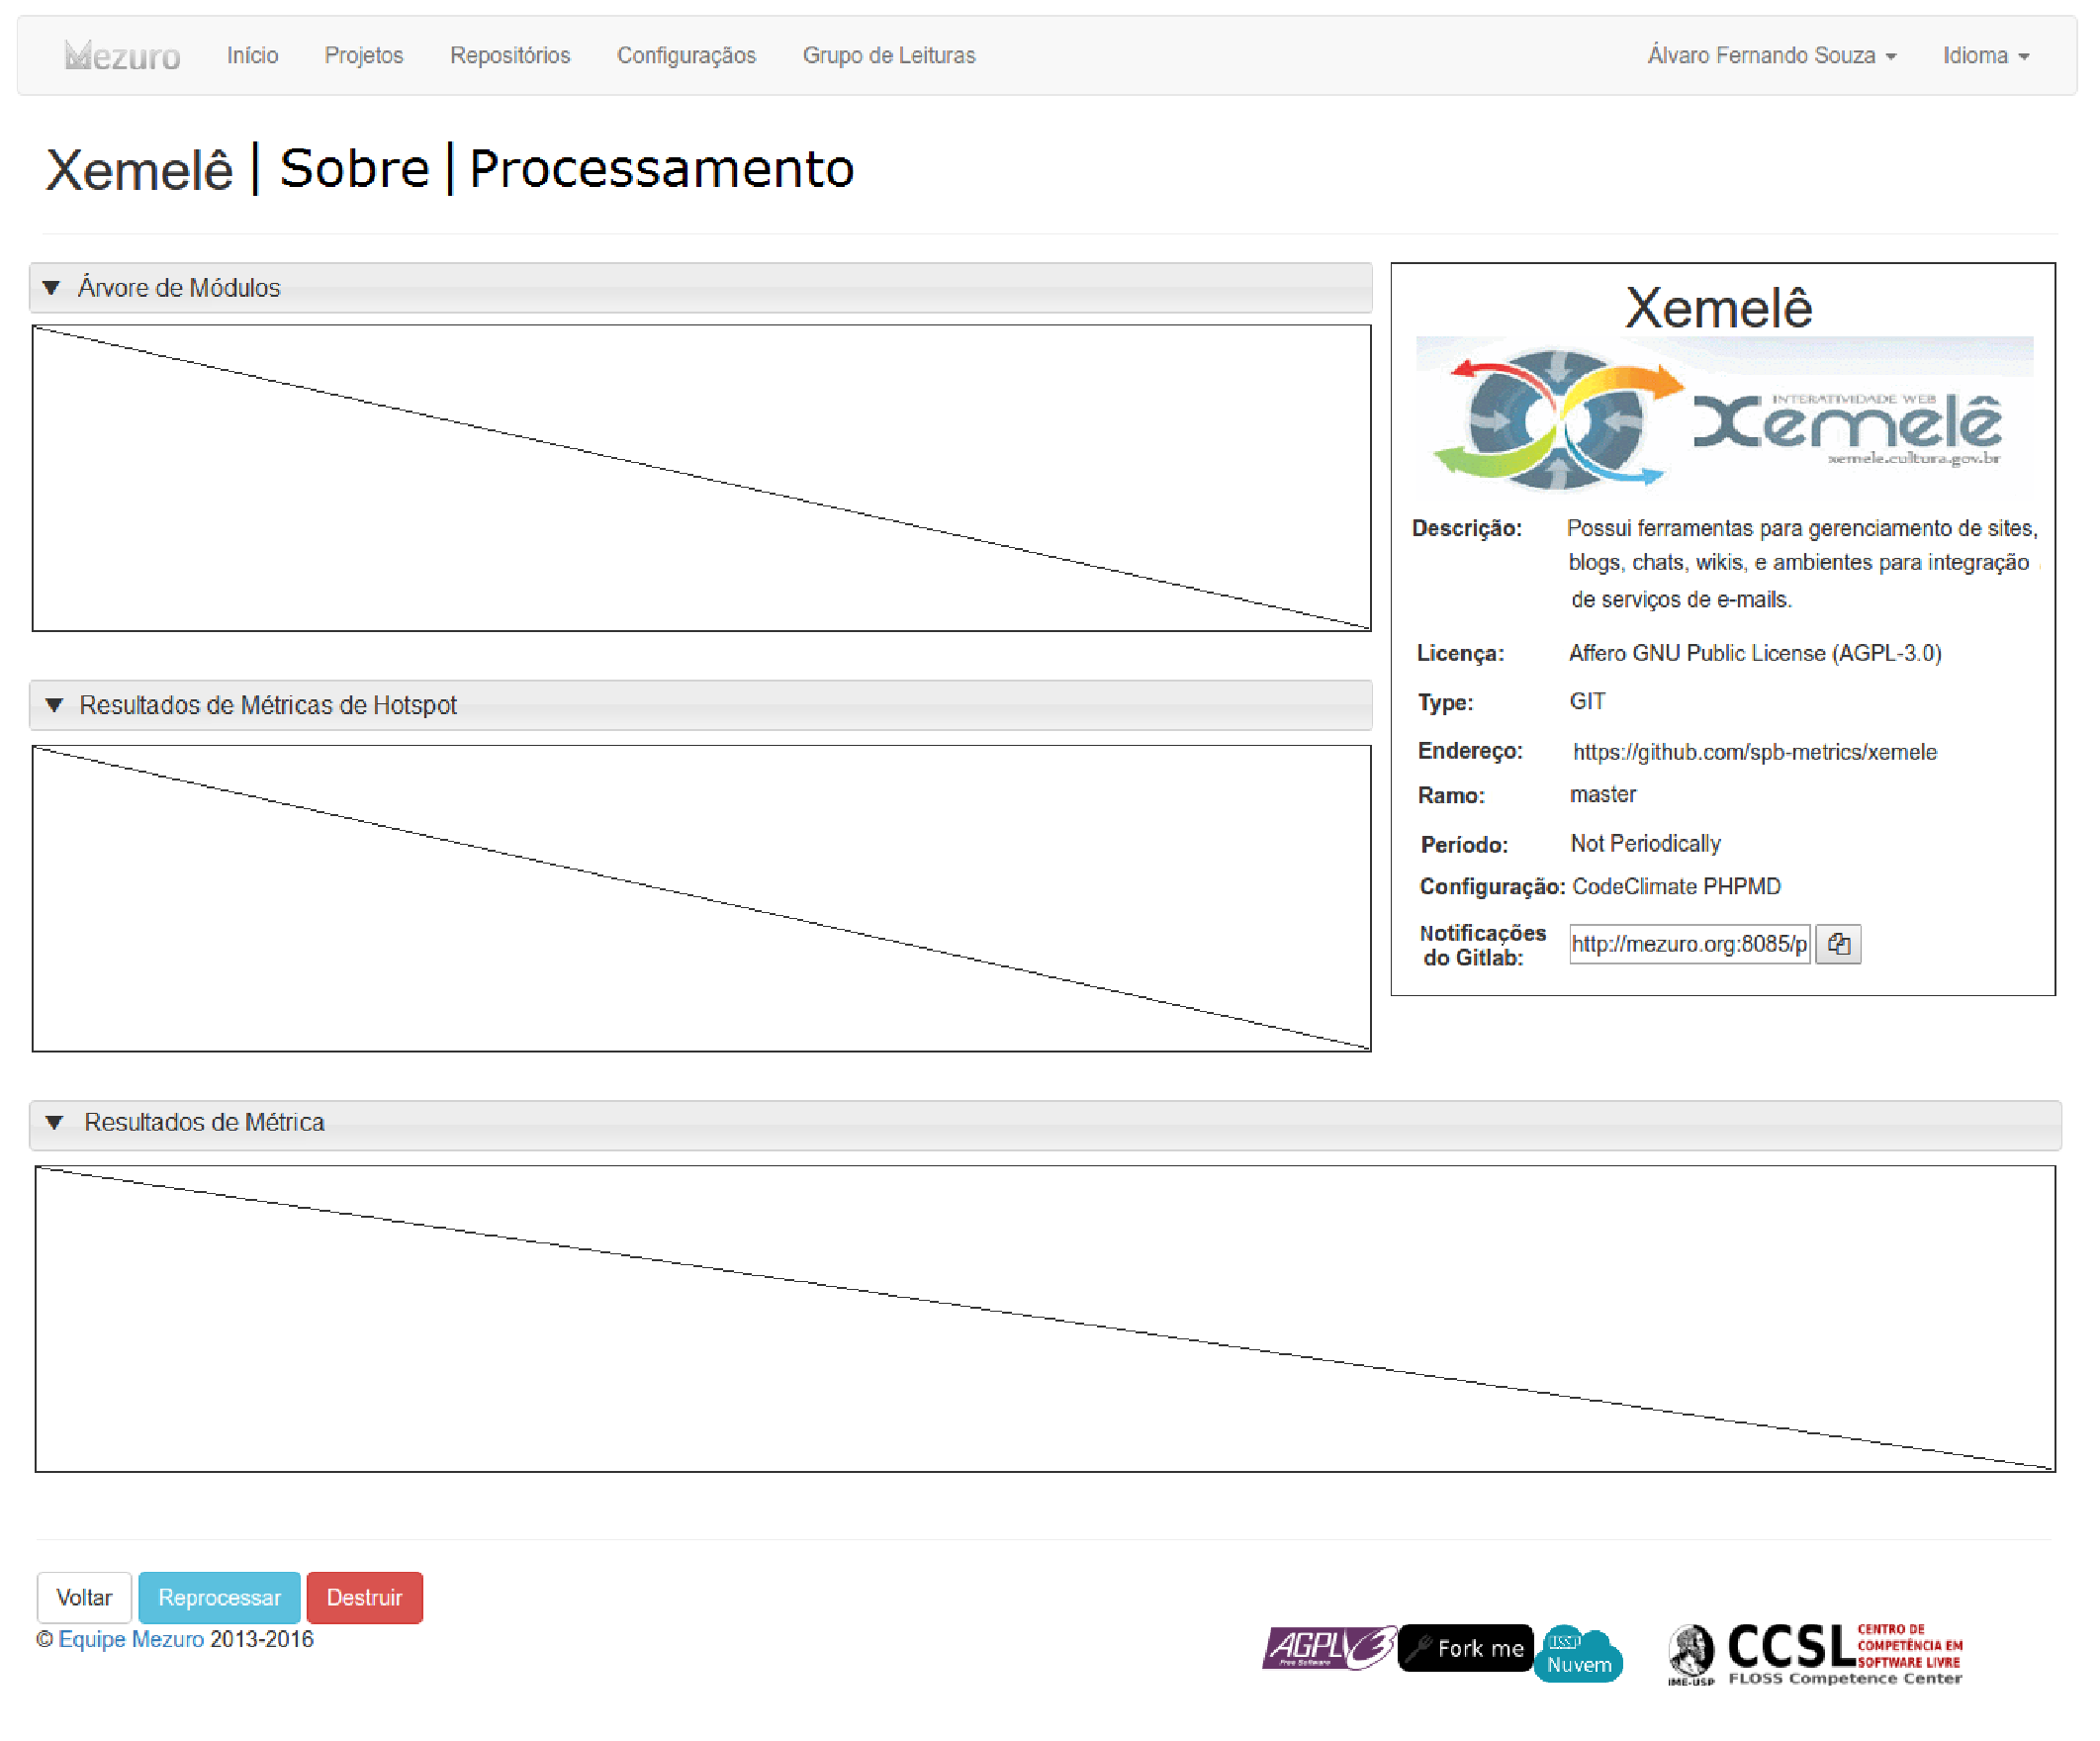
\includegraphics[keepaspectratio=true,scale=0.45]
    {figuras/mezuro-repositorio-view-about-right.eps}
  \caption{Proposta 1 - Informações à direita}
  \label{fig:mezuro-repositorio-view-about-right}
\end{figure}

\newpage

A Figura \ref{fig:mezuro-repositorio-view-about-right} mostra a proposta de
posicionar as informações sobre o repositório, na tela de exibição dos
resultados à direita e trazer o que é mais importante para a avaliação do código
para o topo da tela. Também é proposto a subdivisão das informações ``Sobre''
e as ``Informações de Processamento'' para os menus dispostos ao lado do título
do Software, e cada um sendo um aba de conteúdo. A primeira para os resultados,
a segunda contendo as informações gerais do repositório e a terceira com as
informações de processamento.

\begin{figure}[!htb]
	\centering
    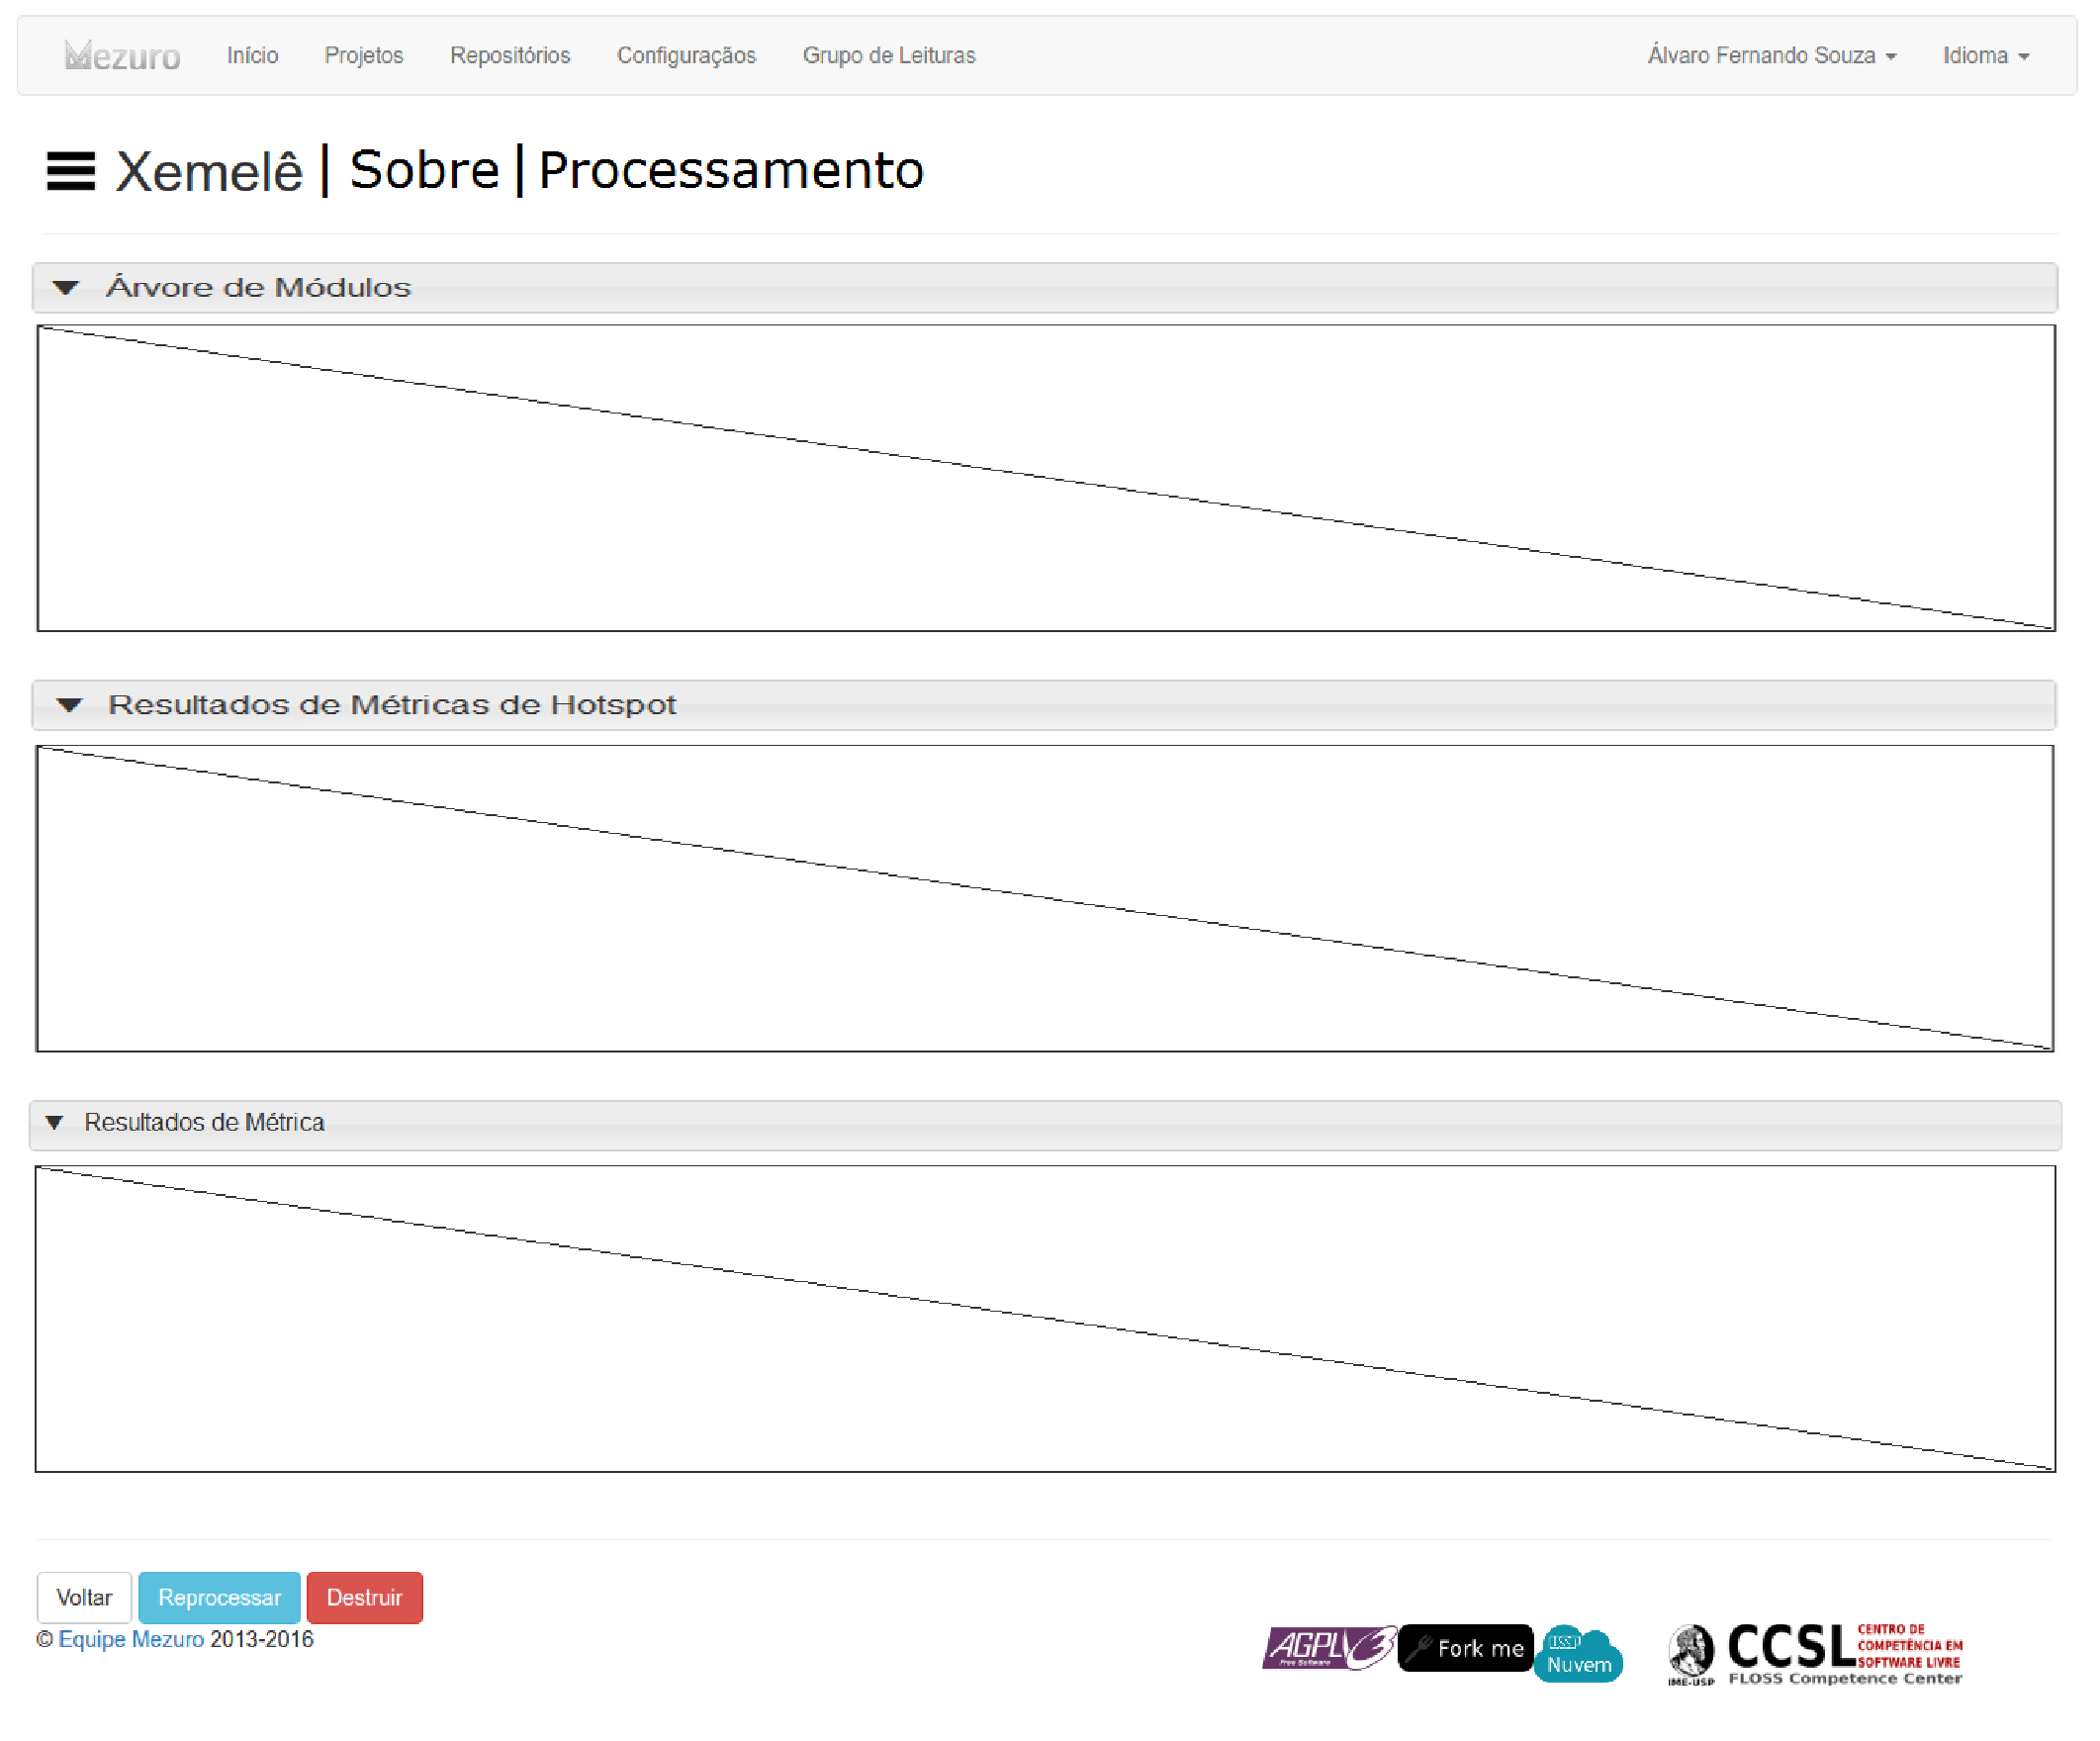
\includegraphics[keepaspectratio=true,scale=0.35]
    {figuras/mezuro-repositorio-view-hamburguer-close.eps}
  \caption{Proposta 2.1 - Informações escondidas - \textit{Menu Hamburger}}
  \label{fig:mezuro-repositorio-view-hamburguer-close}
\end{figure}

\begin{figure}[!htb]
	\centering
    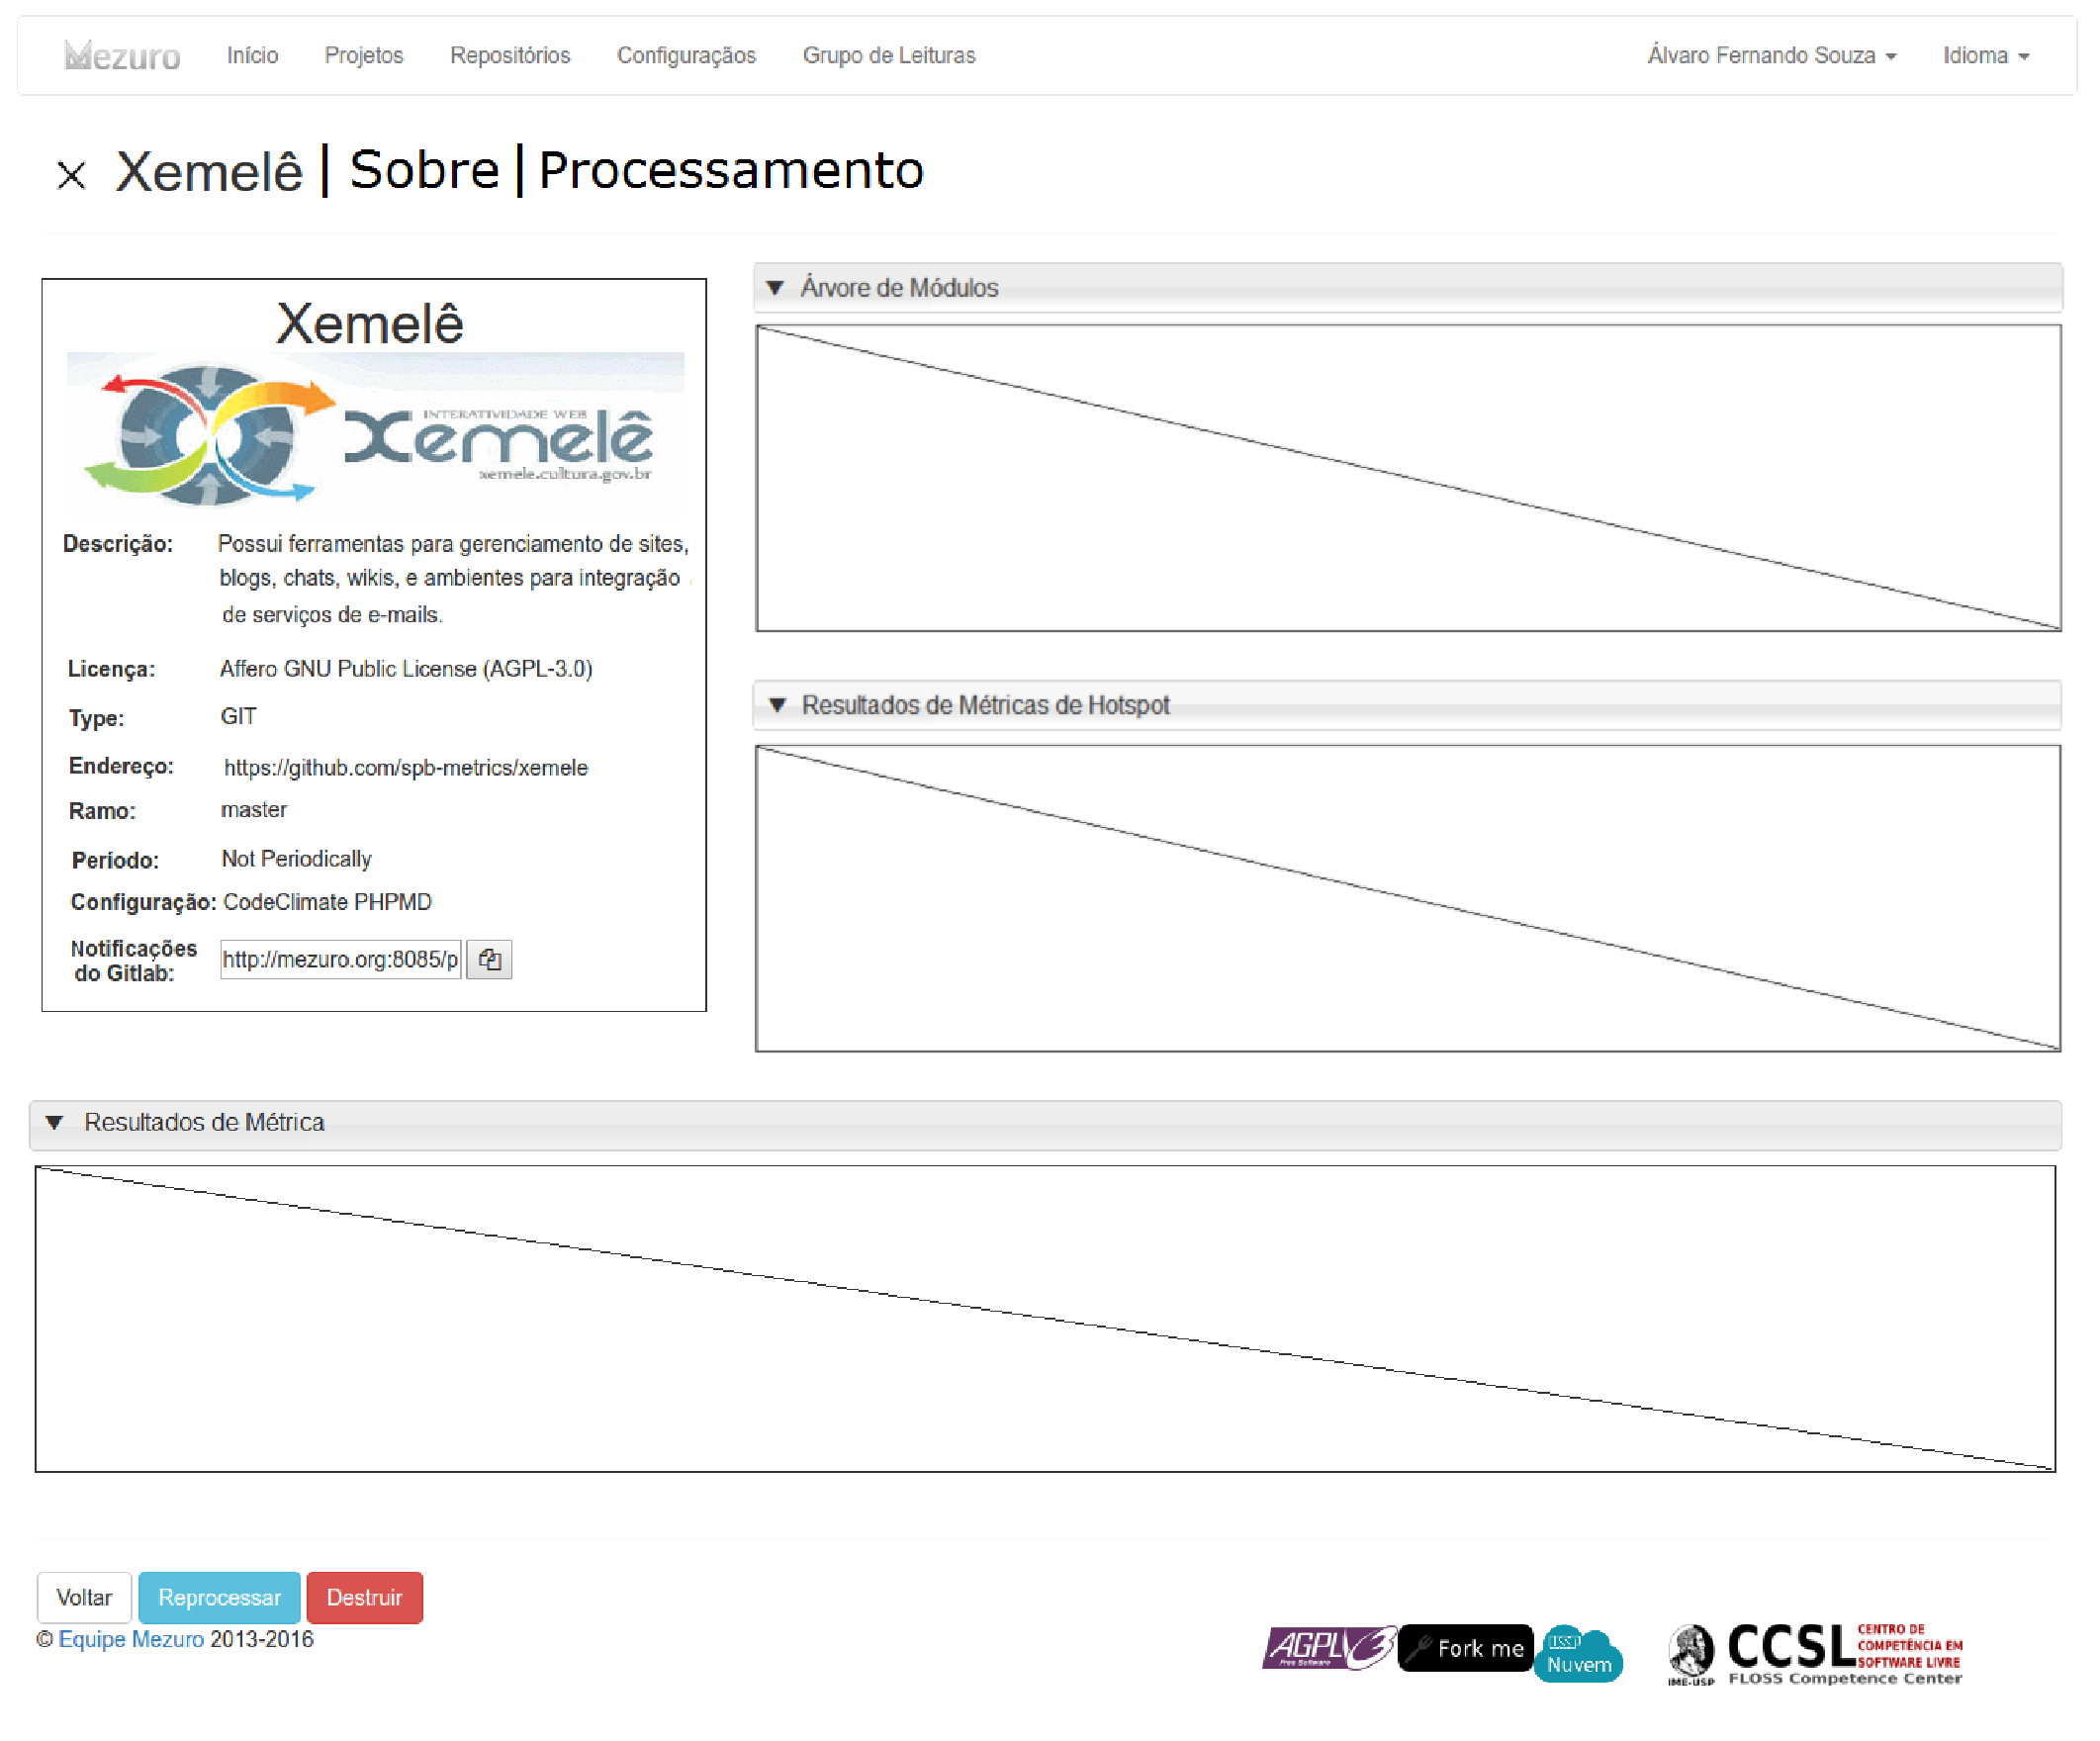
\includegraphics[keepaspectratio=true,scale=0.35]
    {figuras/mezuro-repositorio-view-hamburguer-open.eps}
  \caption{Proposta 2.2 - Informações expostas - \textit{Menu Hamburger}}
  \label{fig:mezuro-repositorio-view-hamburguer-open}
\end{figure}

\newpage

As propostas das Figuras \ref{fig:mezuro-repositorio-view-hamburguer-close} e
\ref{fig:mezuro-repositorio-view-hamburguer-open} são uma possível solução para
novamente trazer o que há de mais importante na avaliação, que são as métricas.
As informações, portanto, ficariam escondidas e acessíveis através do menu
\textit{hamburger} do lado esquerdo do nome do repositório. Ao clicar, o
conteúdo da página afastaria o suficiente para expor as informações e o menu
seria substituído por um símbolo de fechar (letra X).

\begin{figure}[!htb]
	\centering
    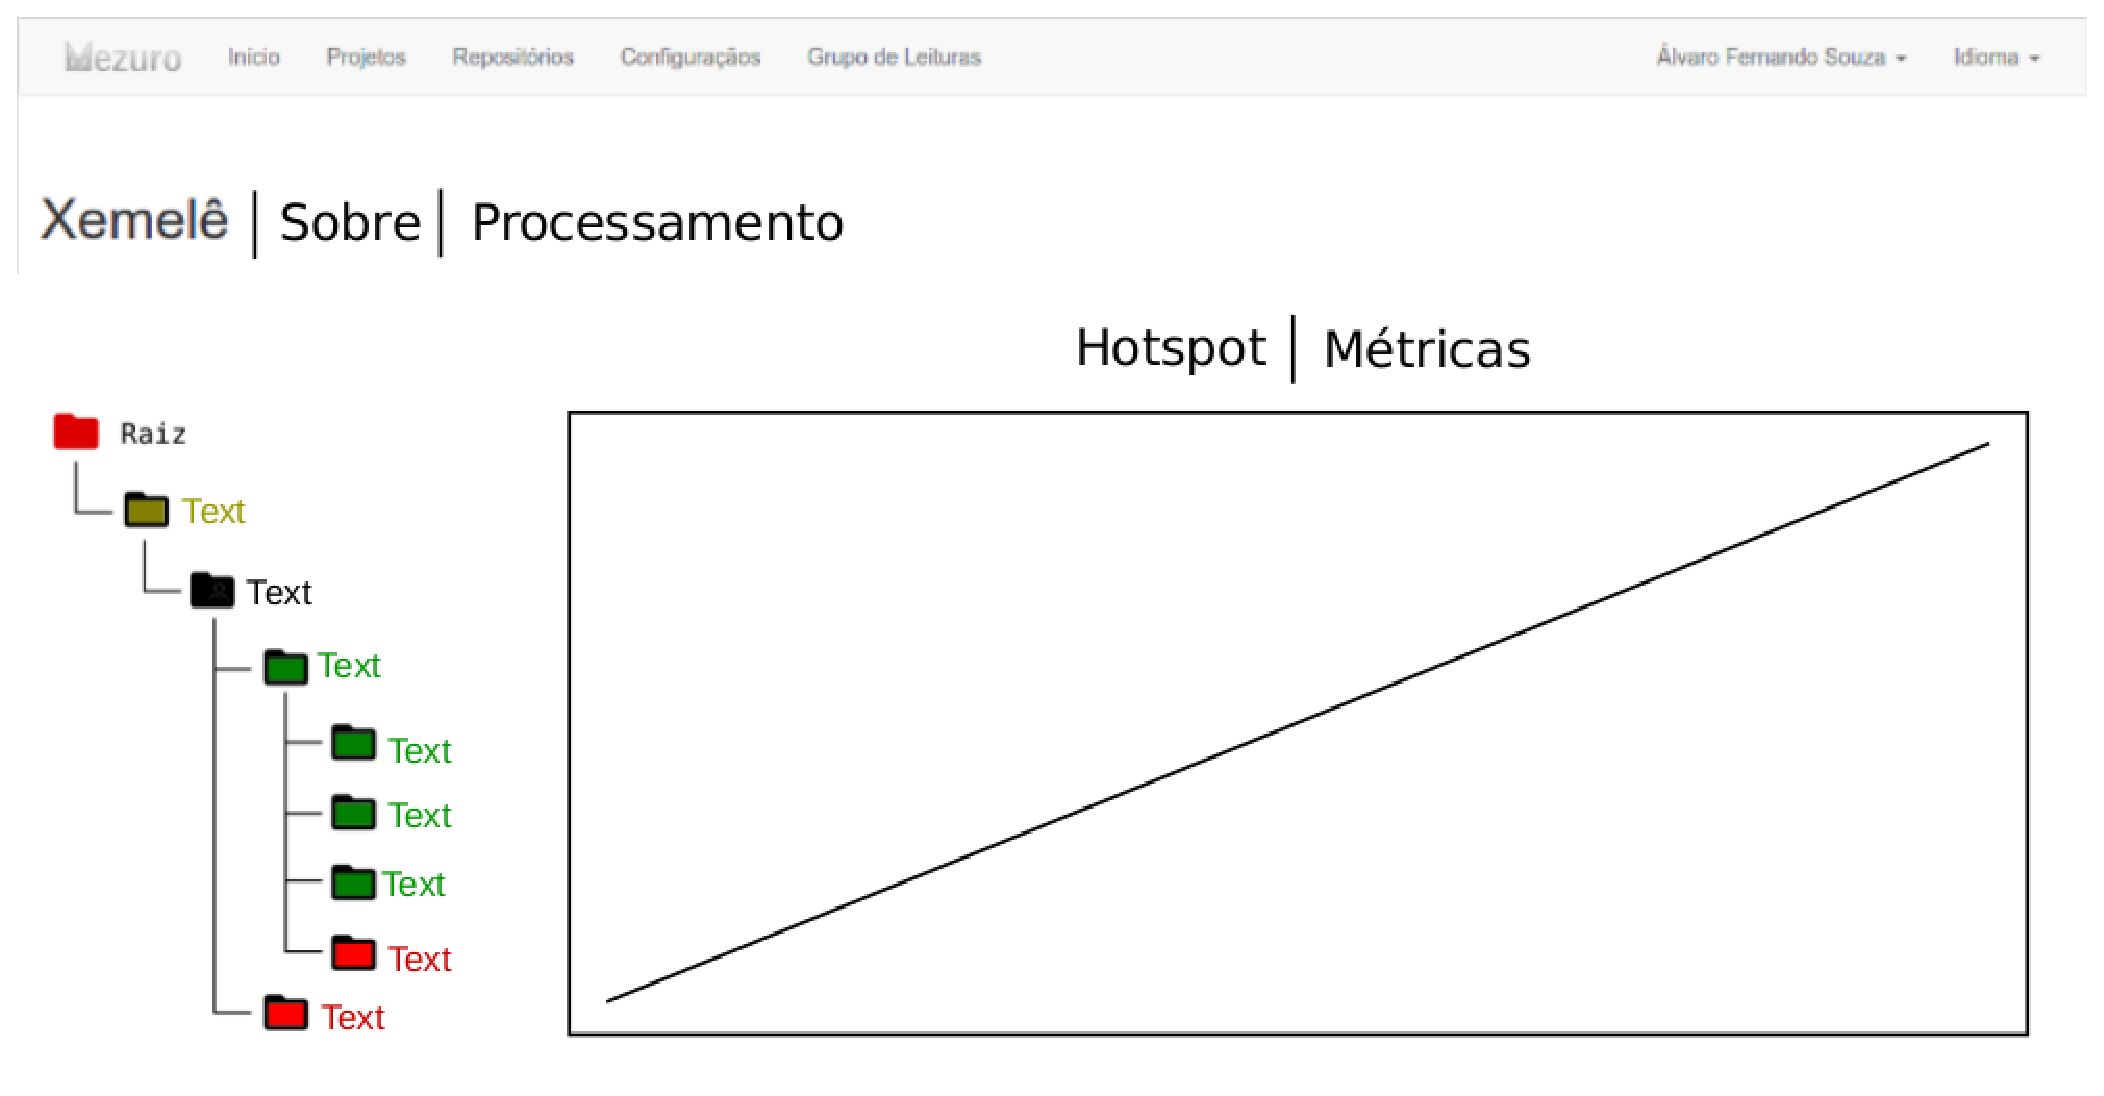
\includegraphics[keepaspectratio=true,scale=0.45]
    {figuras/arvore-lateral.eps}
  \caption{Proposta 3 - Árvore de Módulos na lateral esquerda}
  \label{fig:arvore-lateral}
\end{figure}

A última proposta de evolução da exibição dos resultados no Mezuro, é a exposta
na Figura \ref{fig:arvore-lateral}. A sugestão é: trazer a ``Árvore de Módulos''
já construída na ferramenta, para a esquerda e construí-la de forma semelhante
à estrutura de editores de código-fonte comumente utilizado por desenvolvedores.
Outro ponto importante nessa nova disposição, seria a inclusão das cores de
destaque, que veriam de acordo com as cores já definidas no ``Grupo de Leitura''
e representariam os diretórios/arquivos críticos. Outra proposta é dividir cada
uma das métricas em abas centralizadas e divididas por uma barra vertical.

\begin{figure}[!htb]
	\centering
    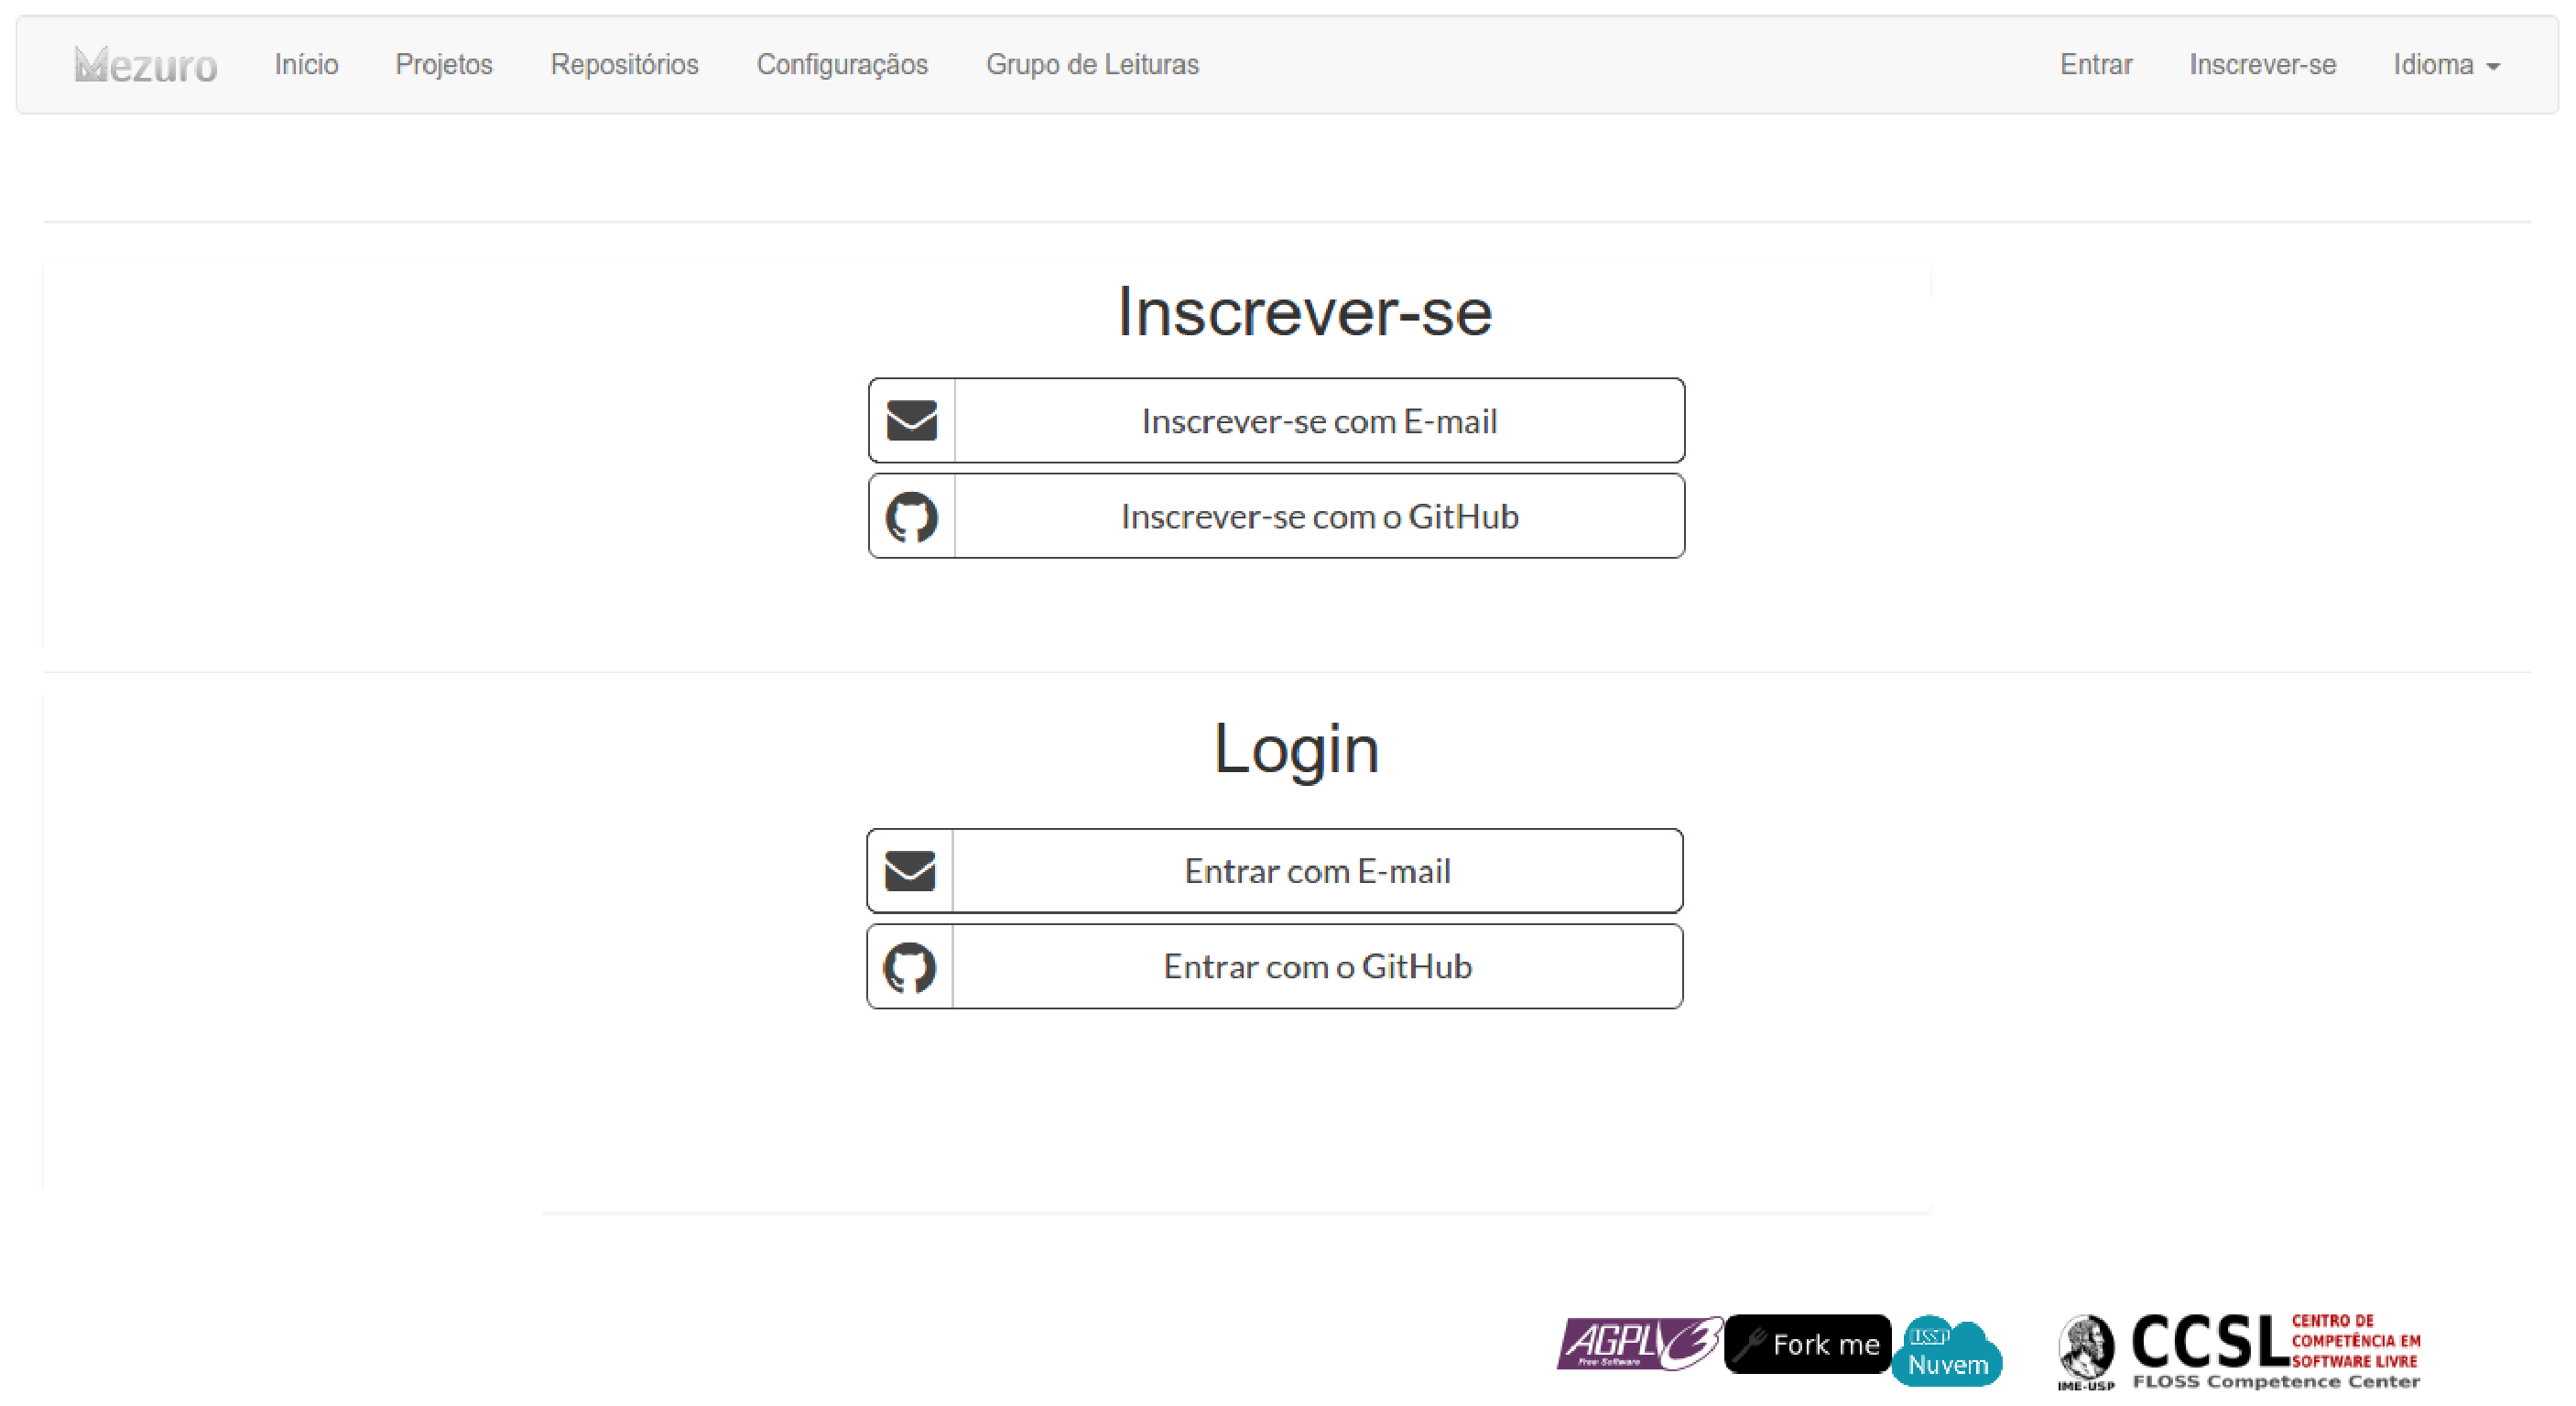
\includegraphics[keepaspectratio=true,scale=0.35]
    {figuras/mezuro-cadastro-github.eps}
  \caption{Proposta 4.1 - Cadastro e \textit{Login} com o Github}
  \label{fig:mezuro-cadastro-github}
\end{figure}

\begin{figure}[!htb]
	\centering
    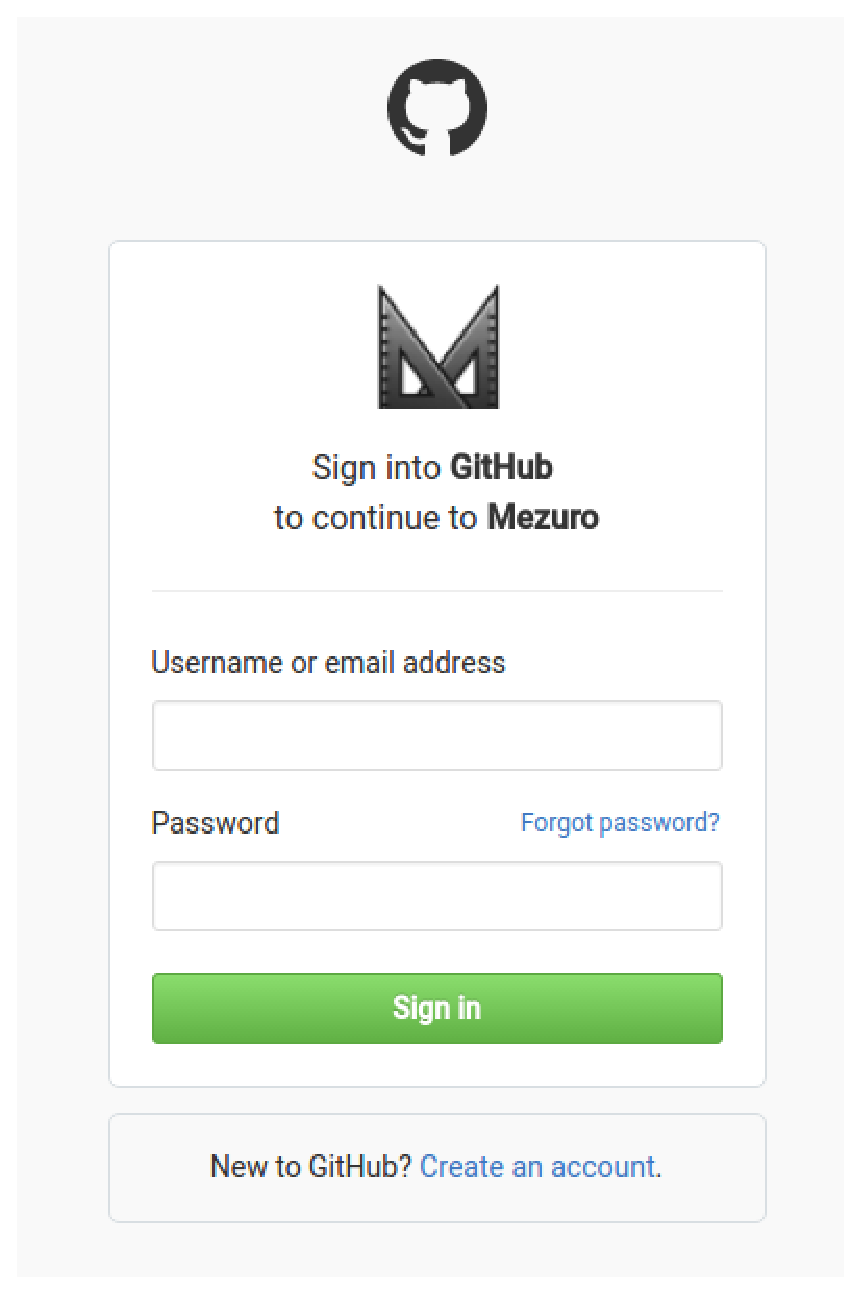
\includegraphics[keepaspectratio=true,scale=0.5]
    {figuras/singup_mezuro_github.eps}
  \caption{Proposta 4.2 - Tela de \textit{Login} no Github}
  \label{fig:singup_mezuro_github}
\end{figure}

Também  são propostas telas relacionadas com a interação do usuário e com o
objetivo de tornar o Mezuro mais atrativo a novos usuários.
%
A Figura \ref{fig:mezuro-cadastro-github} mostra a proposta de opção ao usuário
de realizar o cadastro e o \textit{login} com a conta do Github ou com e-mail.
E a Figura \ref{fig:singup_mezuro_github} mostra como seria a interação com o
usuário na tela de \textit{login} gerada pelo próprio Github.

\begin{figure}[!htb]
	\centering
    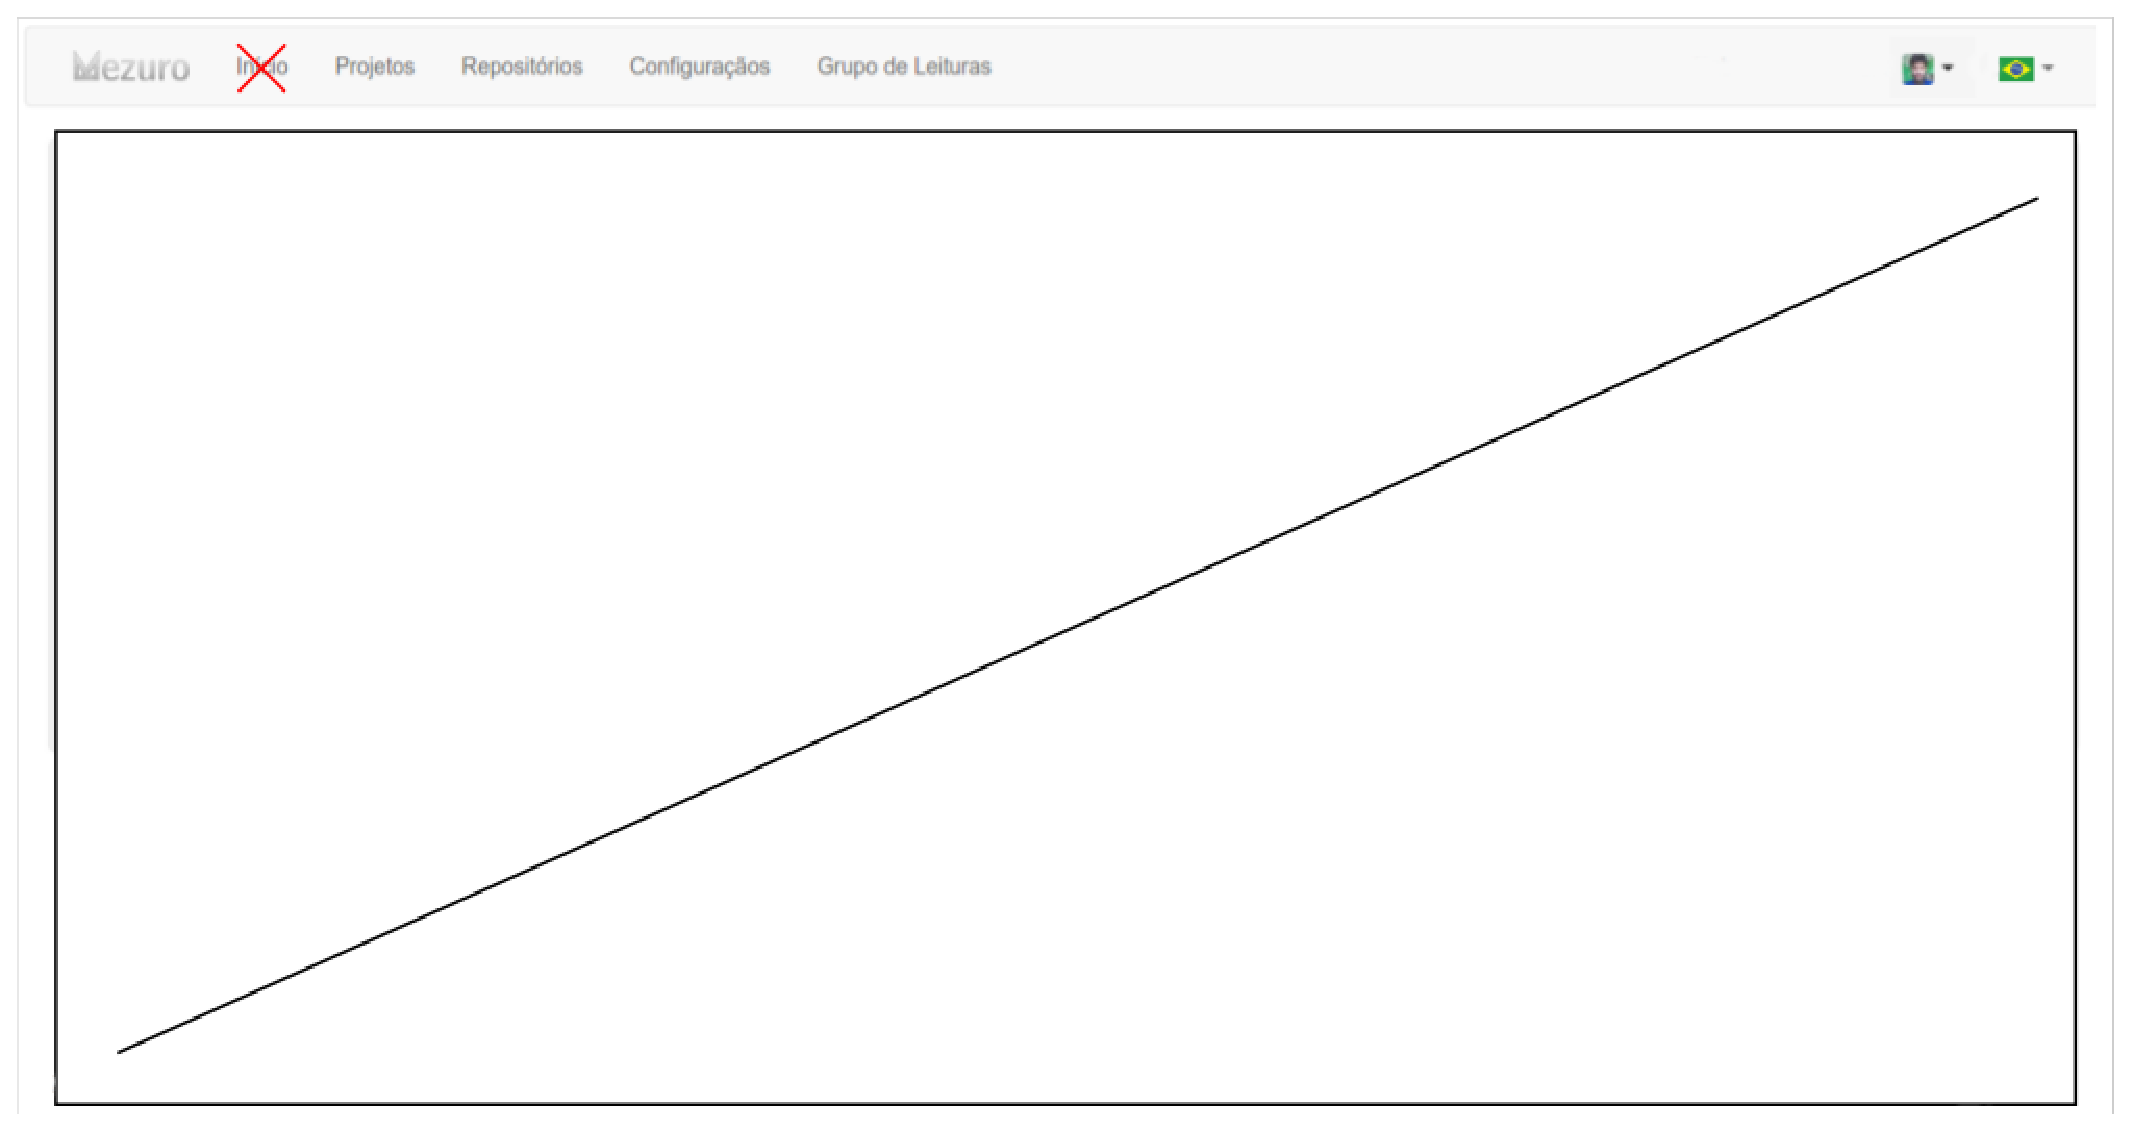
\includegraphics[keepaspectratio=true,scale=0.45]
    {figuras/barra-superior.eps}
  \caption{Proposta 5 - Nova Barra Superior}
  \label{fig:barra-superior}
\end{figure}

A proposta da Figura \ref{fig:barra-superior} demonstra a modificação dos
seguintes aspectos: imagem do usuário (vinda do Gravatar ou da conta do Github)
ao invés do nome literal; modificação do texto da linguagem para a bandeira da
nação correspondente; e retirada do menu ``Início'', pois já é uma convenção de
páginas \textit{Webs} que a imagem do site seja o retorno para o seu início.
O aluno acredita que a foto do usuário irá trazer mais pessoalidade e avivamento
ao Mezuro.

\begin{figure}[!htb]
	\centering
    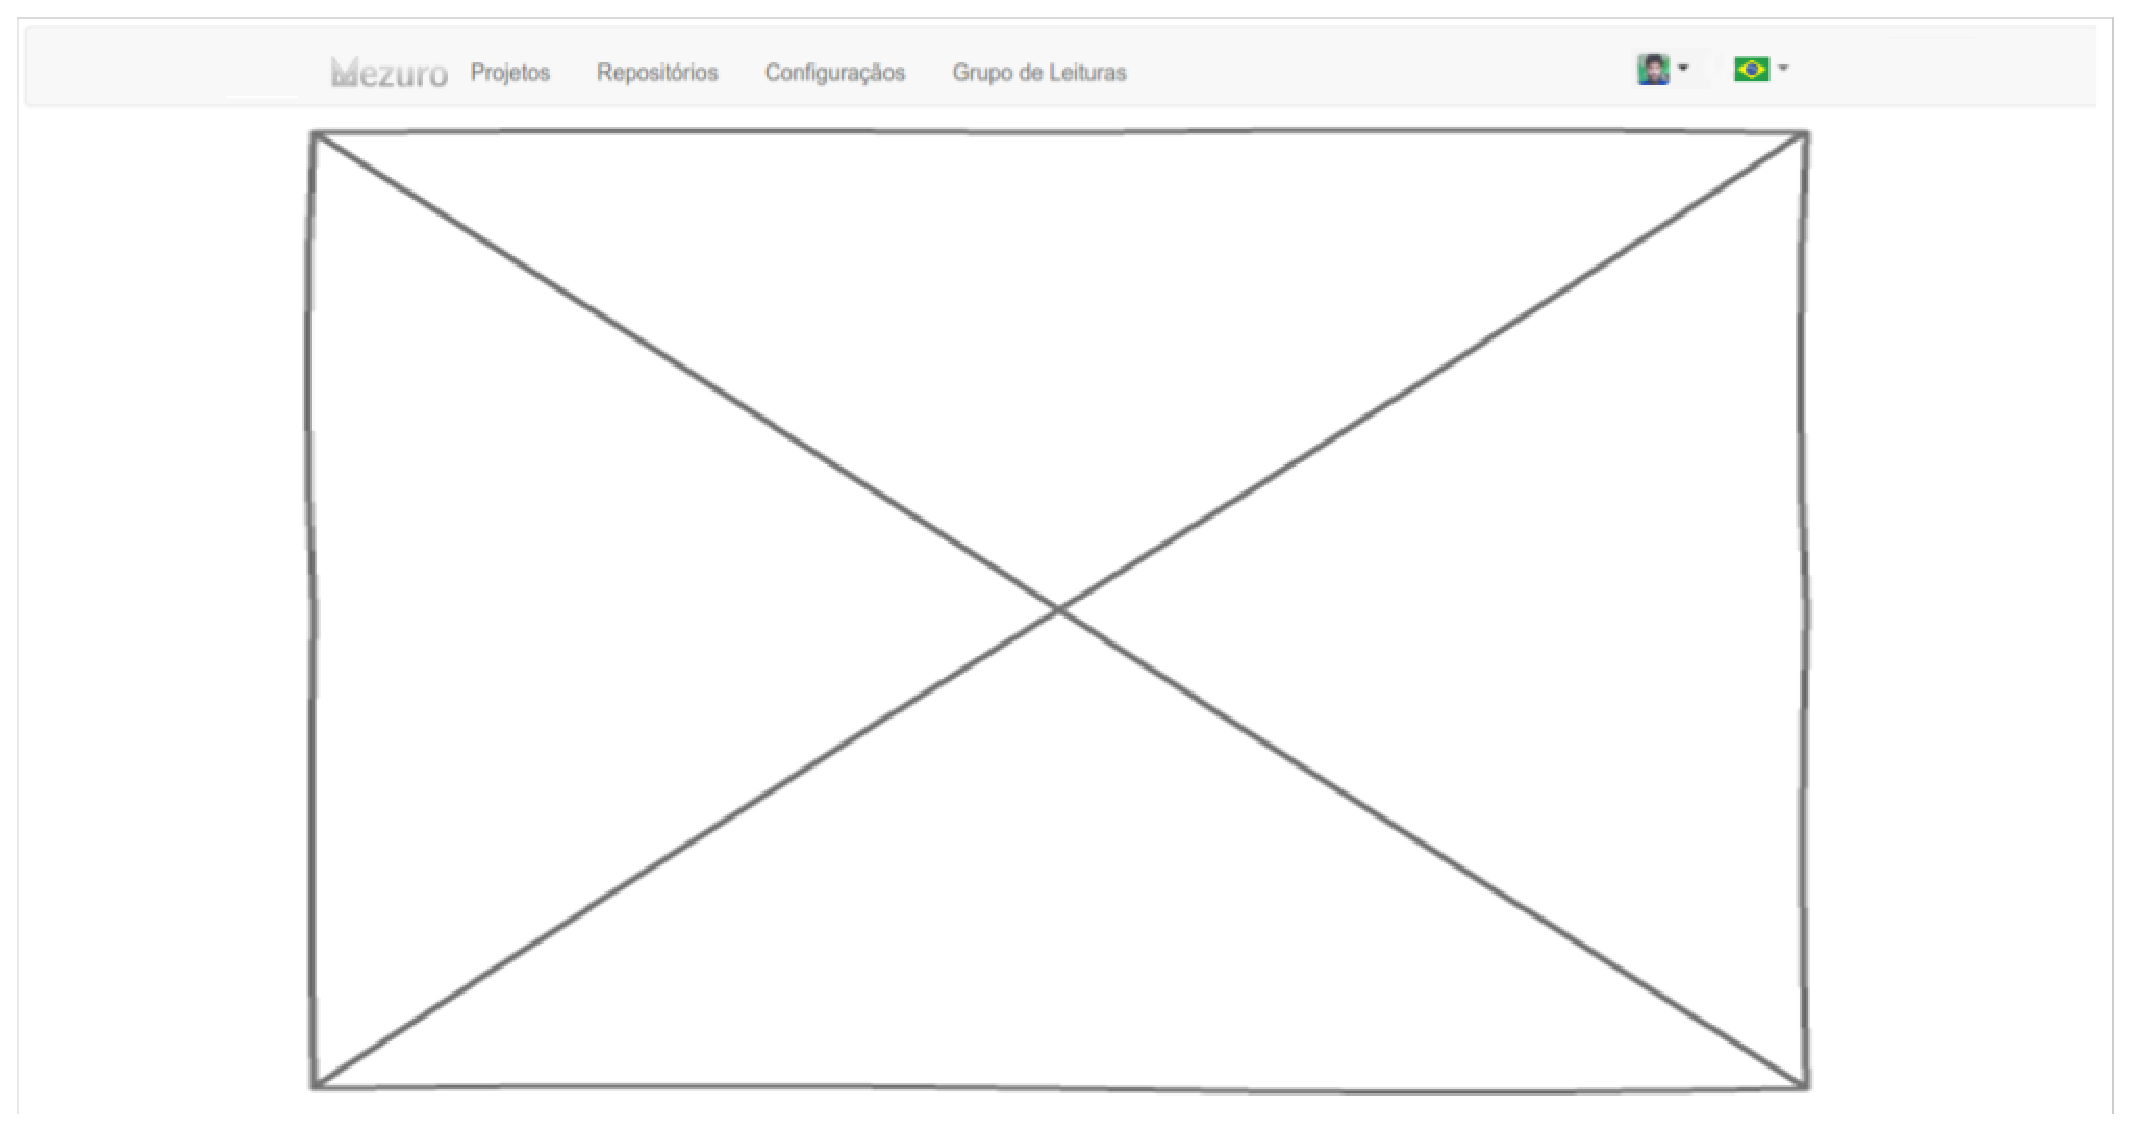
\includegraphics[keepaspectratio=true,scale=0.45]
    {figuras/size_content_1.eps}
  \caption{Proposta 6 - Largura da disposição do conteúdo}
  \label{fig:size_content_1}
\end{figure}

\newpage

A última proposta, Figura \ref{fig:size_content_1}, visa sugerir a diminuição da
largura em que o conteúdo do site é exposto. A disposição seria então
centralizada, com o tamanho de 960px em uma tela de 1320px disponíveis, cerca de
72\% da tela. Nas versões para \textit{tablets} e celulares, essa proporção de
largura poderia ocupar 100\% da tela.

% Seção 6.2 - Discussão/Avaliação de técnicas de VS no Mezuro
% "existe essa proposta do experimento, mas não recomendamos no momento..."

\section{Avaliação de Técnicas de VS no Mezuro}

Nesta seção é exposto: o exemplo de uso utilizando a biblioteca Javascript D3.js;
as justificativas e escolhas de projetos para este exemplo; e a exposição da
pesquisa de avaliação feita com estudantes e pessoas envolvidas com o
desenvolvimento do Mezuro.

\subsection{D3 - Data-Driven Documents}

D3.js (\textit{Data-Driven-Documents}) é uma biblioteca Javascript construída
inicialmente por \citeonline{bostock2011d3}, que tem como um dos seus objetivos
principais a produção de visualizações dinâmicas e interativas para a \textit{Web}. Ela
faz uso de várias tecnologias vastamente utilizadas: HTML (para o conteúdo das
páginas), SVG (para descrição de gráficos vetoriais) e CSS (para estética das
páginas). A Figura \ref{fig:d3_gears} é um exemplo de como esse uso (ou
interação) é feito. Esta biblioteca permite ao programador manipular o Modelo de
Objeto de Documento (do inglês, \textit{Document Object Model} - DOM), para
modificar determinada seleção de elementos na página. Essa modificação, seja
adição ou remoção de elementos, depende dos dados de entrada e é onde a
aplicação de transformações dinâmicas é feita. Os autores idealizaram a união de
três preocupações: compatibilidade, depuração e desempenho \cite{bostock2011d3}.

\begin{figure}[!htb]
	\centering
    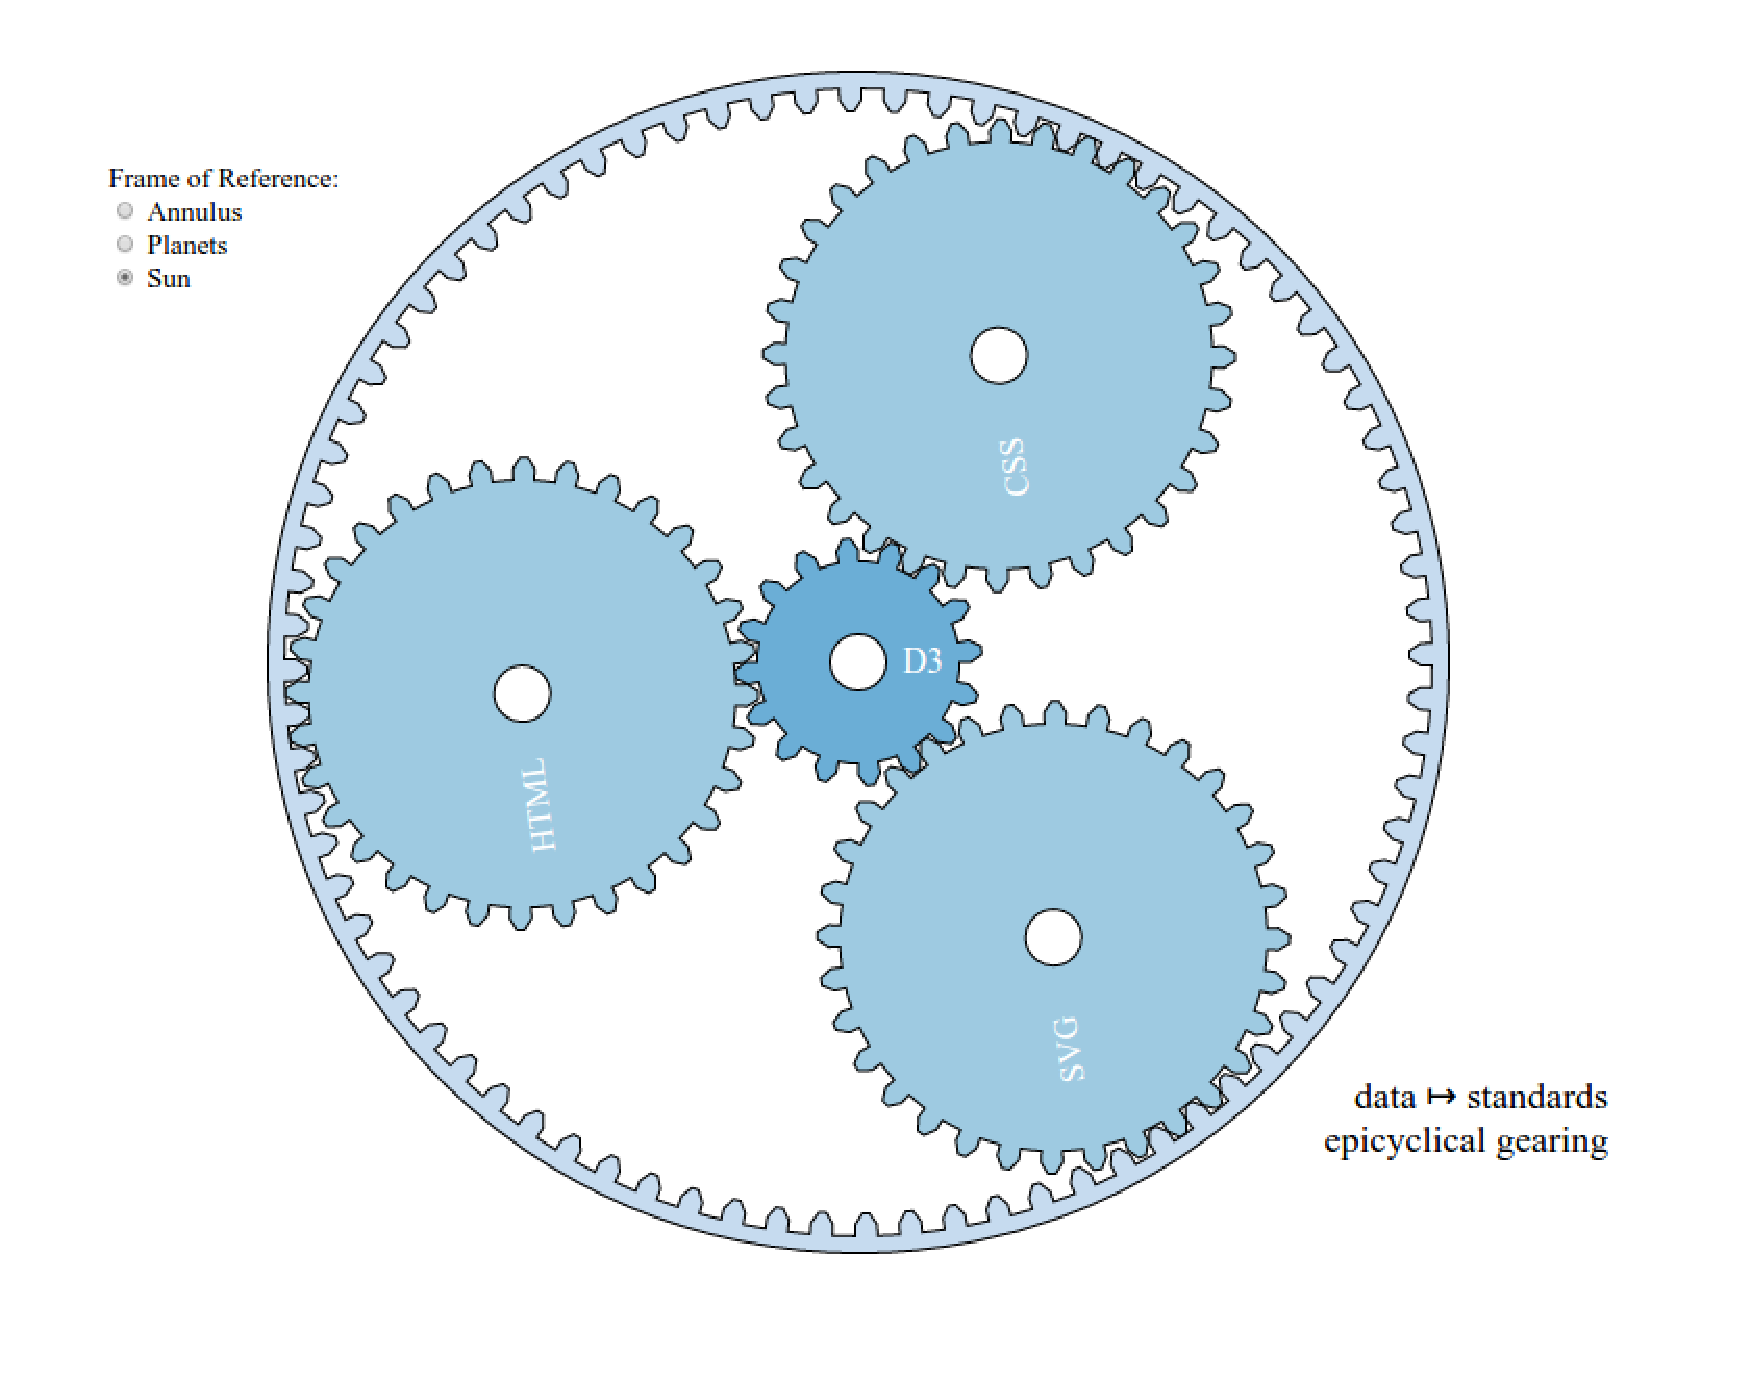
\includegraphics[keepaspectratio=true,scale=0.5]
    {figuras/d3_gears.eps}
  \caption{Exemplificação do Uso das Tecnologias pela D3.js \cite{michaeld3}}
  \label{fig:d3_gears}
\end{figure}

A biblioteca D3.js é licenciada sob a \textit{BSD licenses}, que é compatível
com a licença do Mezuro (\textit{AGPL} - \textit{Version} 3) e possui uma vasta
galeria\footnote{\url{https://github.com/mbostock/d3/wiki/Gallery}} de exemplos
que podem se adaptar ao proposto neste trabalho.

\begin{figure}[!htb]
	\centering
    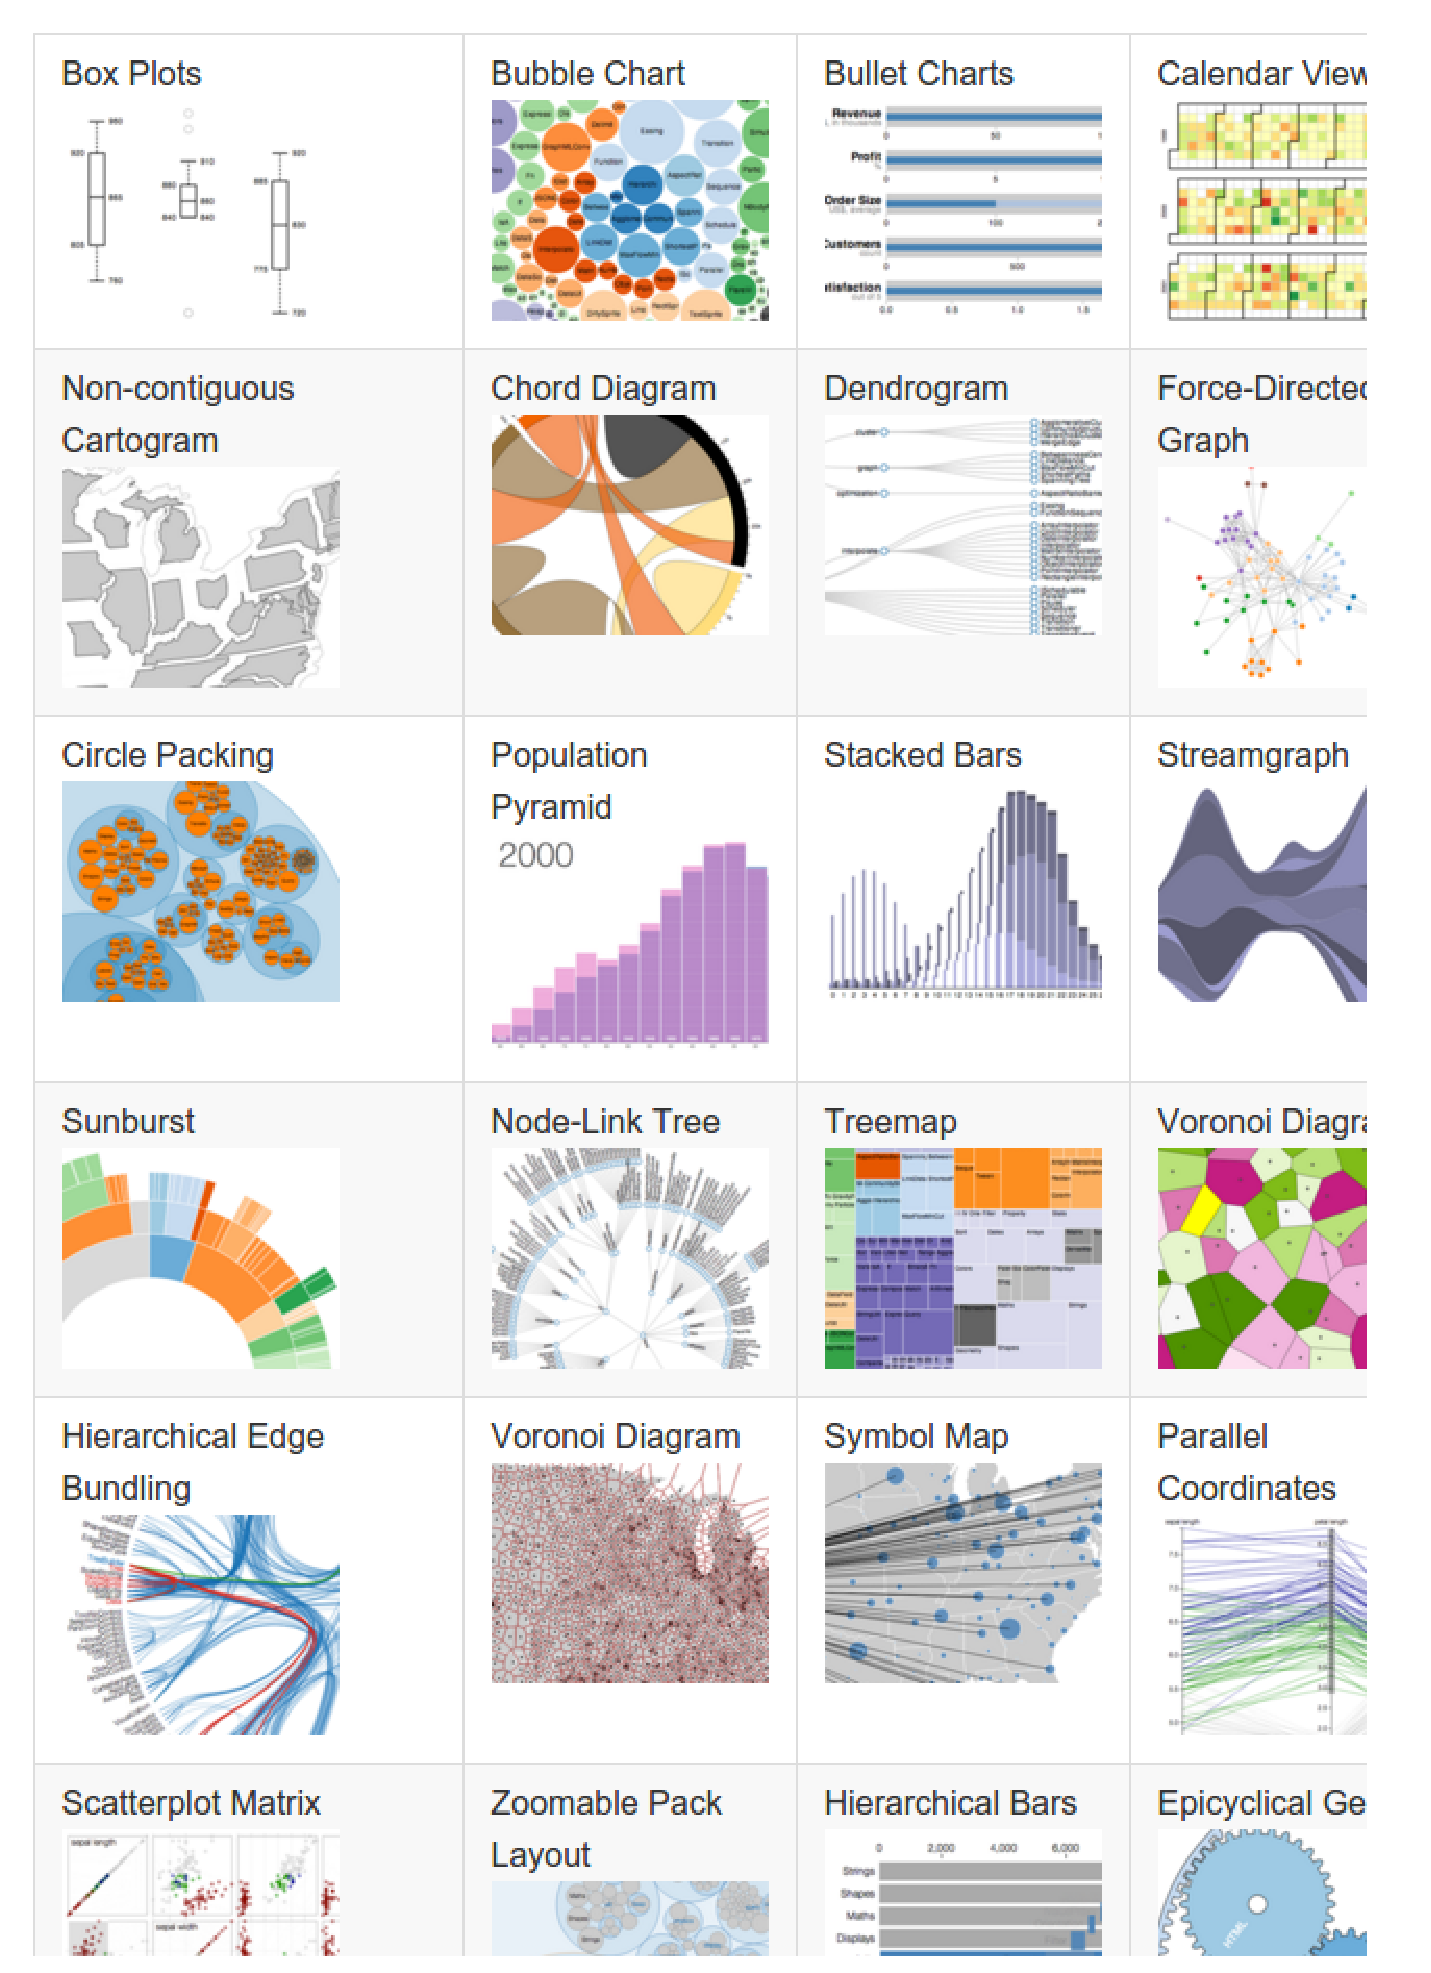
\includegraphics[keepaspectratio=true,scale=0.5]
    {figuras/d3_gallery.eps}
  \caption{Galeria de Exemplos da biblioteca D3.js \cite{galleryD3}}
  \label{fig:d3_gallery}
\end{figure}

\subsection{Exemplo de Uso}

Como prova de conceito, foi realizado a adaptação de três visualizações dos
exemplos disponíveis na galeria da biblioteca D3. A primeira, feita por Thomas
Preusse, tem como título \textit{Radar Chart}
\footnote{\url{http://bl.ocks.org/tpreusse/2bc99d74a461b8c0acb1}}. Nesta
primeira adaptação, os valores de três métricas são gerados aleatoriamente. As
métricas foram escolhidas apenas para fins de ilustração. São elas: número de
métodos, número de métodos públicos e total de módulos.

Para a segunda e terceira adaptações foram coletadas métricas do projeto da
\textit{engine} para jogos, levando-se
em consideração apenas três classes (Animation, MouseButtonEvent e Level). As
métricas são da configuração inicial do Mezuro para projetos Java/C/C++. As
métricas são:

\begin{itemize}
  \item \textbf{ACC} (\textit{Afferent Connections per Class} - Conexões
	aferentes de uma classe)
  \item \textbf{ACCM} (\textit{Average Cyclomatic Complexity per Method} -
	Média da Complexidade Ciclomática por método)
  \item \textbf{AMLOC} (\textit{Average Method LOC} - Média do número de linhas
	de código por método)
  \item \textbf{ANPM} (\textit{Average Number of Parameters per Method} - Média
	do número de linhas de código por método)
  \item \textbf{DIT} (\textit{Depth of Inheritance Tree} - Profundidade da
	árvore de herança)
  \item \textbf{NOM} (\textit{Number of Methods} - Número de métodos)
  \item \textbf{NPA} (\textit{Number of Public Attributes} - Número de
	atributos públicos)
  \item \textbf{SC} (\textit{Structural Complexity} - Complexidade estrutural)
\end{itemize}



\begin{figure}[!htb]
	\centering
    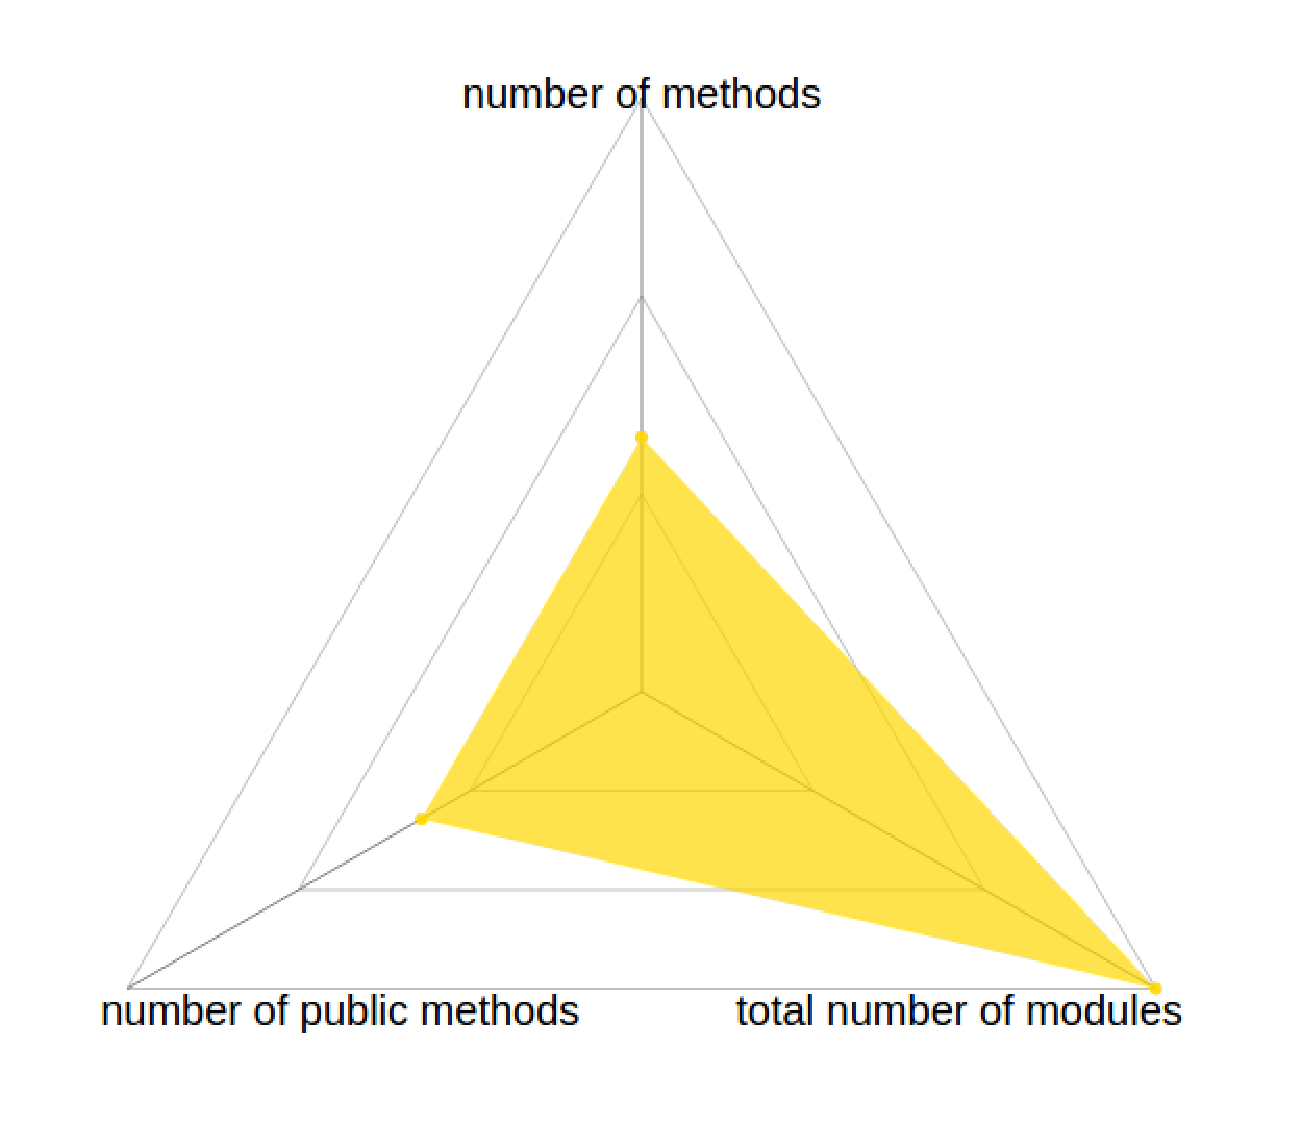
\includegraphics[keepaspectratio=true,scale=0.5]
    {figuras/radar.eps}
  \caption{Gráfico Radar por Thomas Preusse (adaptado)}
  \label{fig:radar}
\end{figure}

\begin{figure}[!htb]
	\centering
    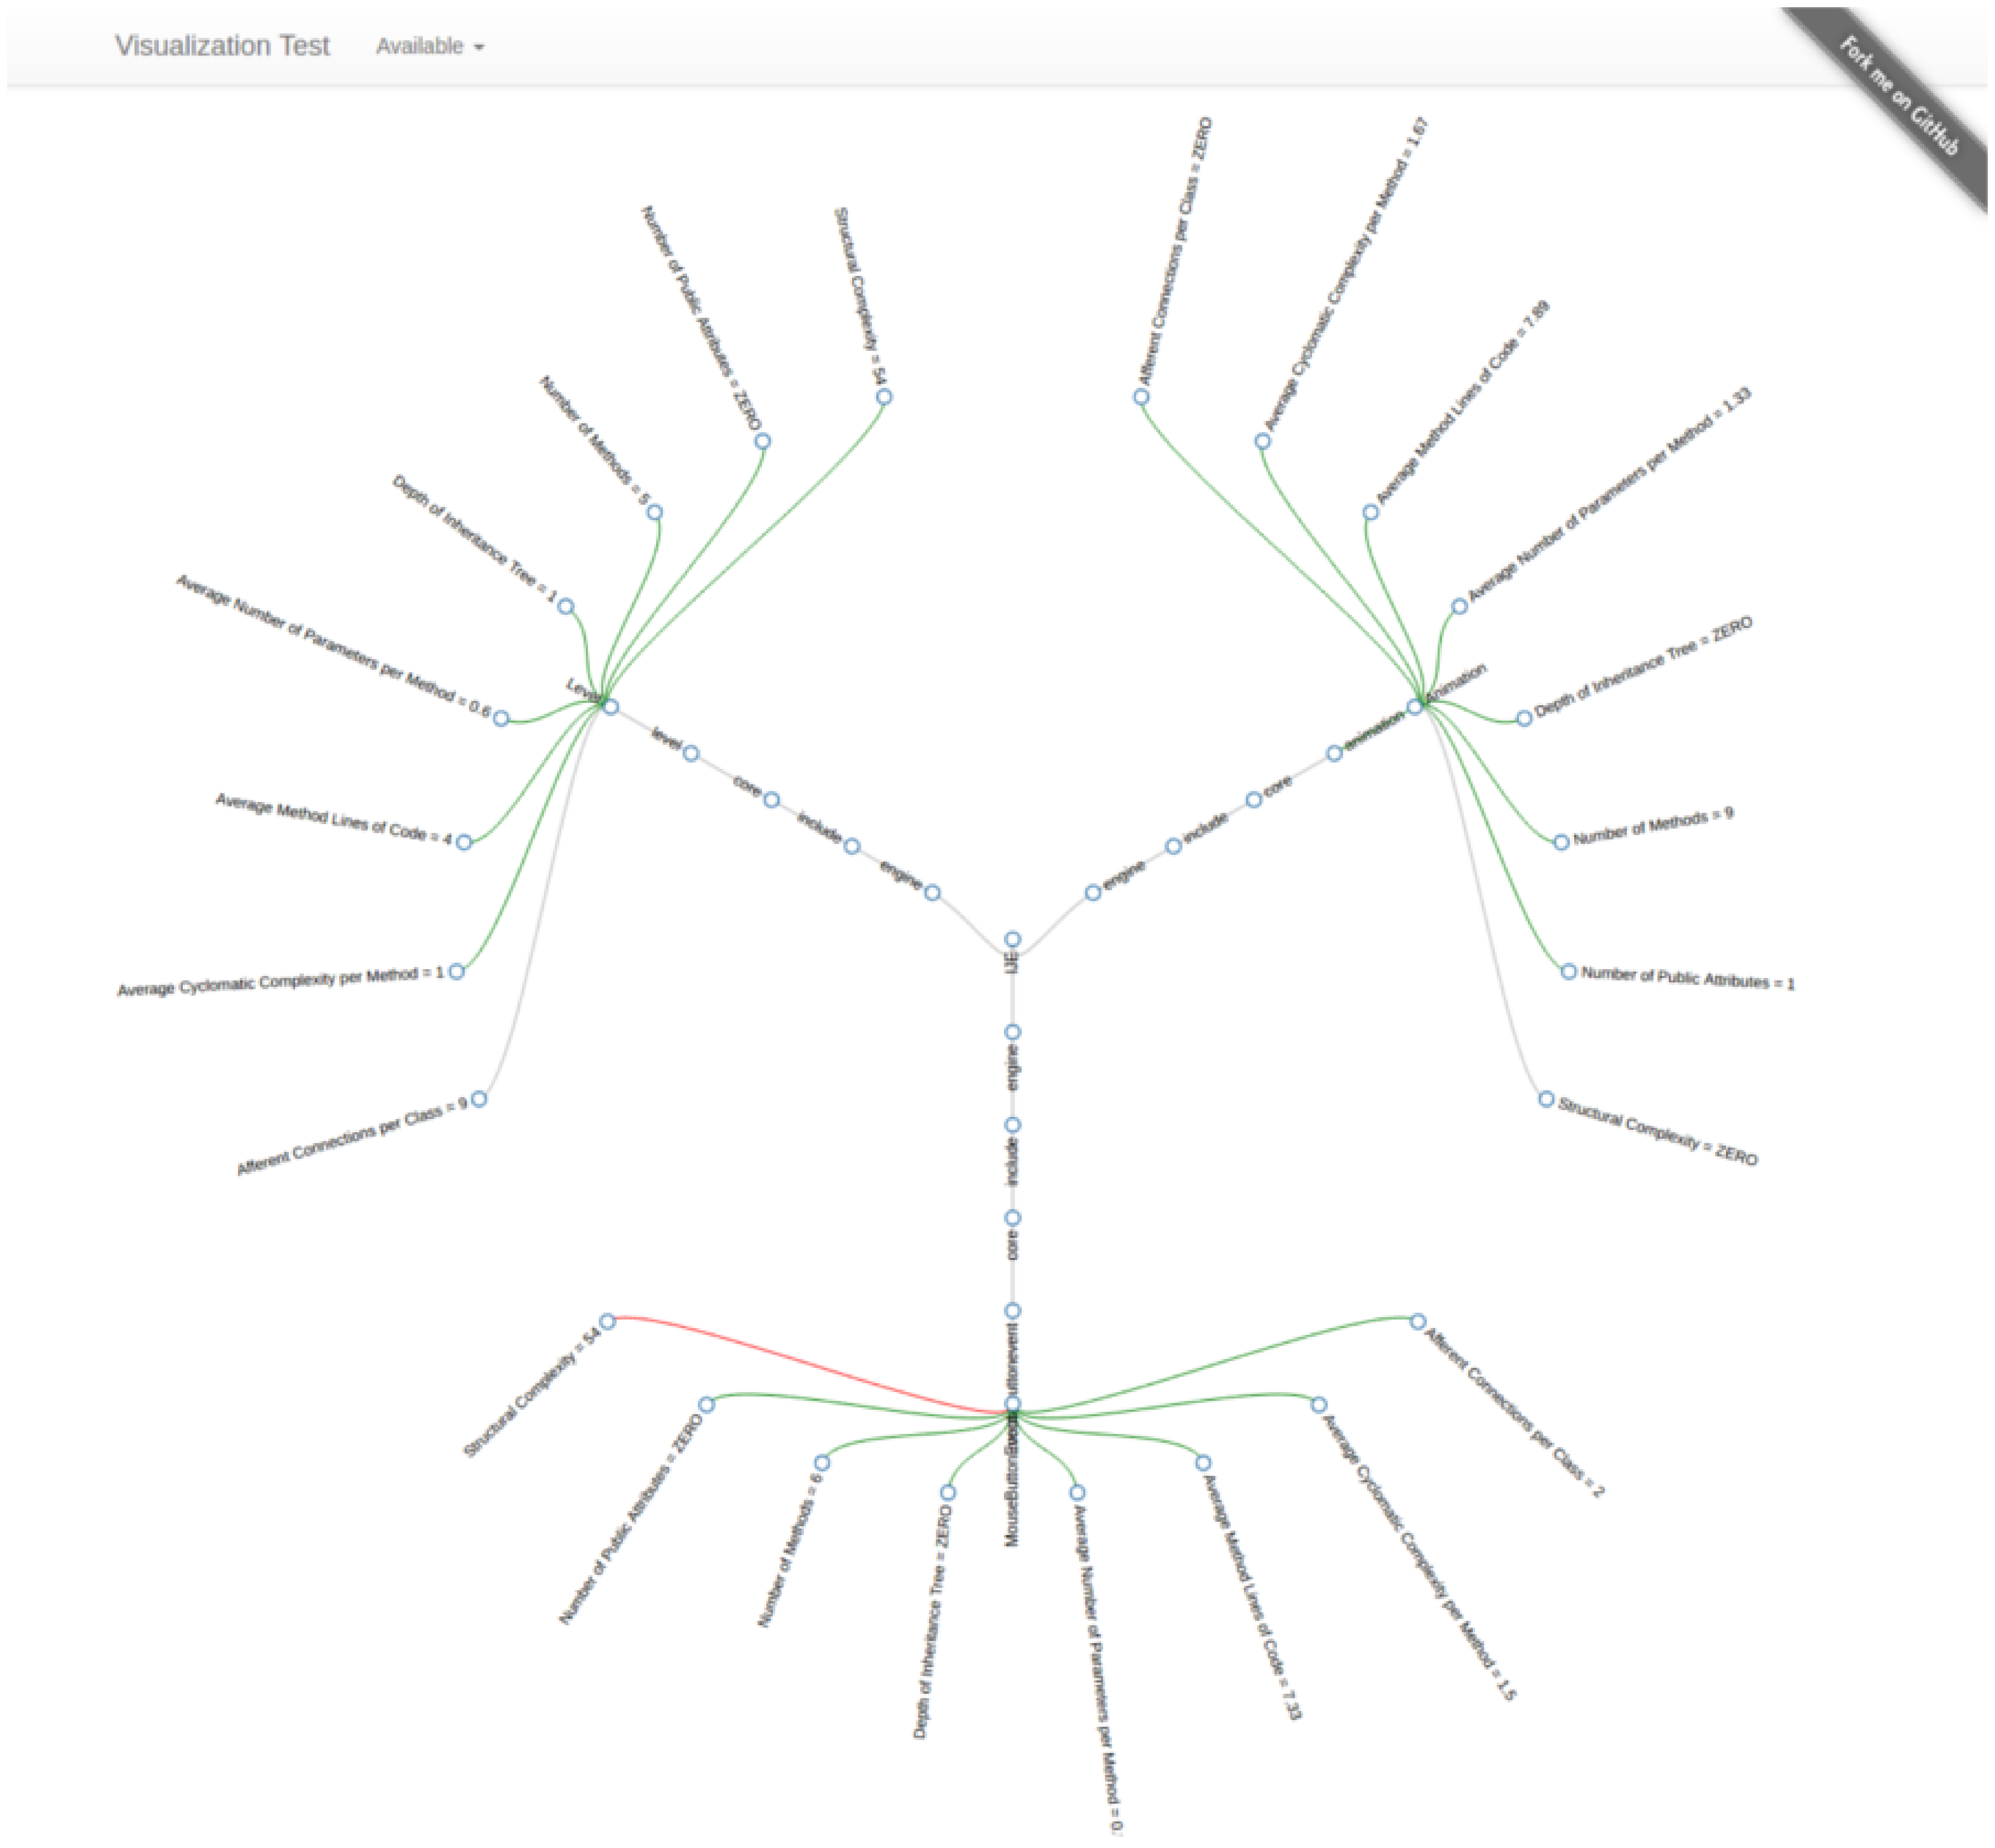
\includegraphics[keepaspectratio=true,scale=0.15]
    {figuras/node_link_tree.eps}
  \caption{Node Link Tree por Michael Bostock (adaptado)}
  \label{fig:node_link_tree}
\end{figure}

\begin{figure}[!htb]
	\centering
    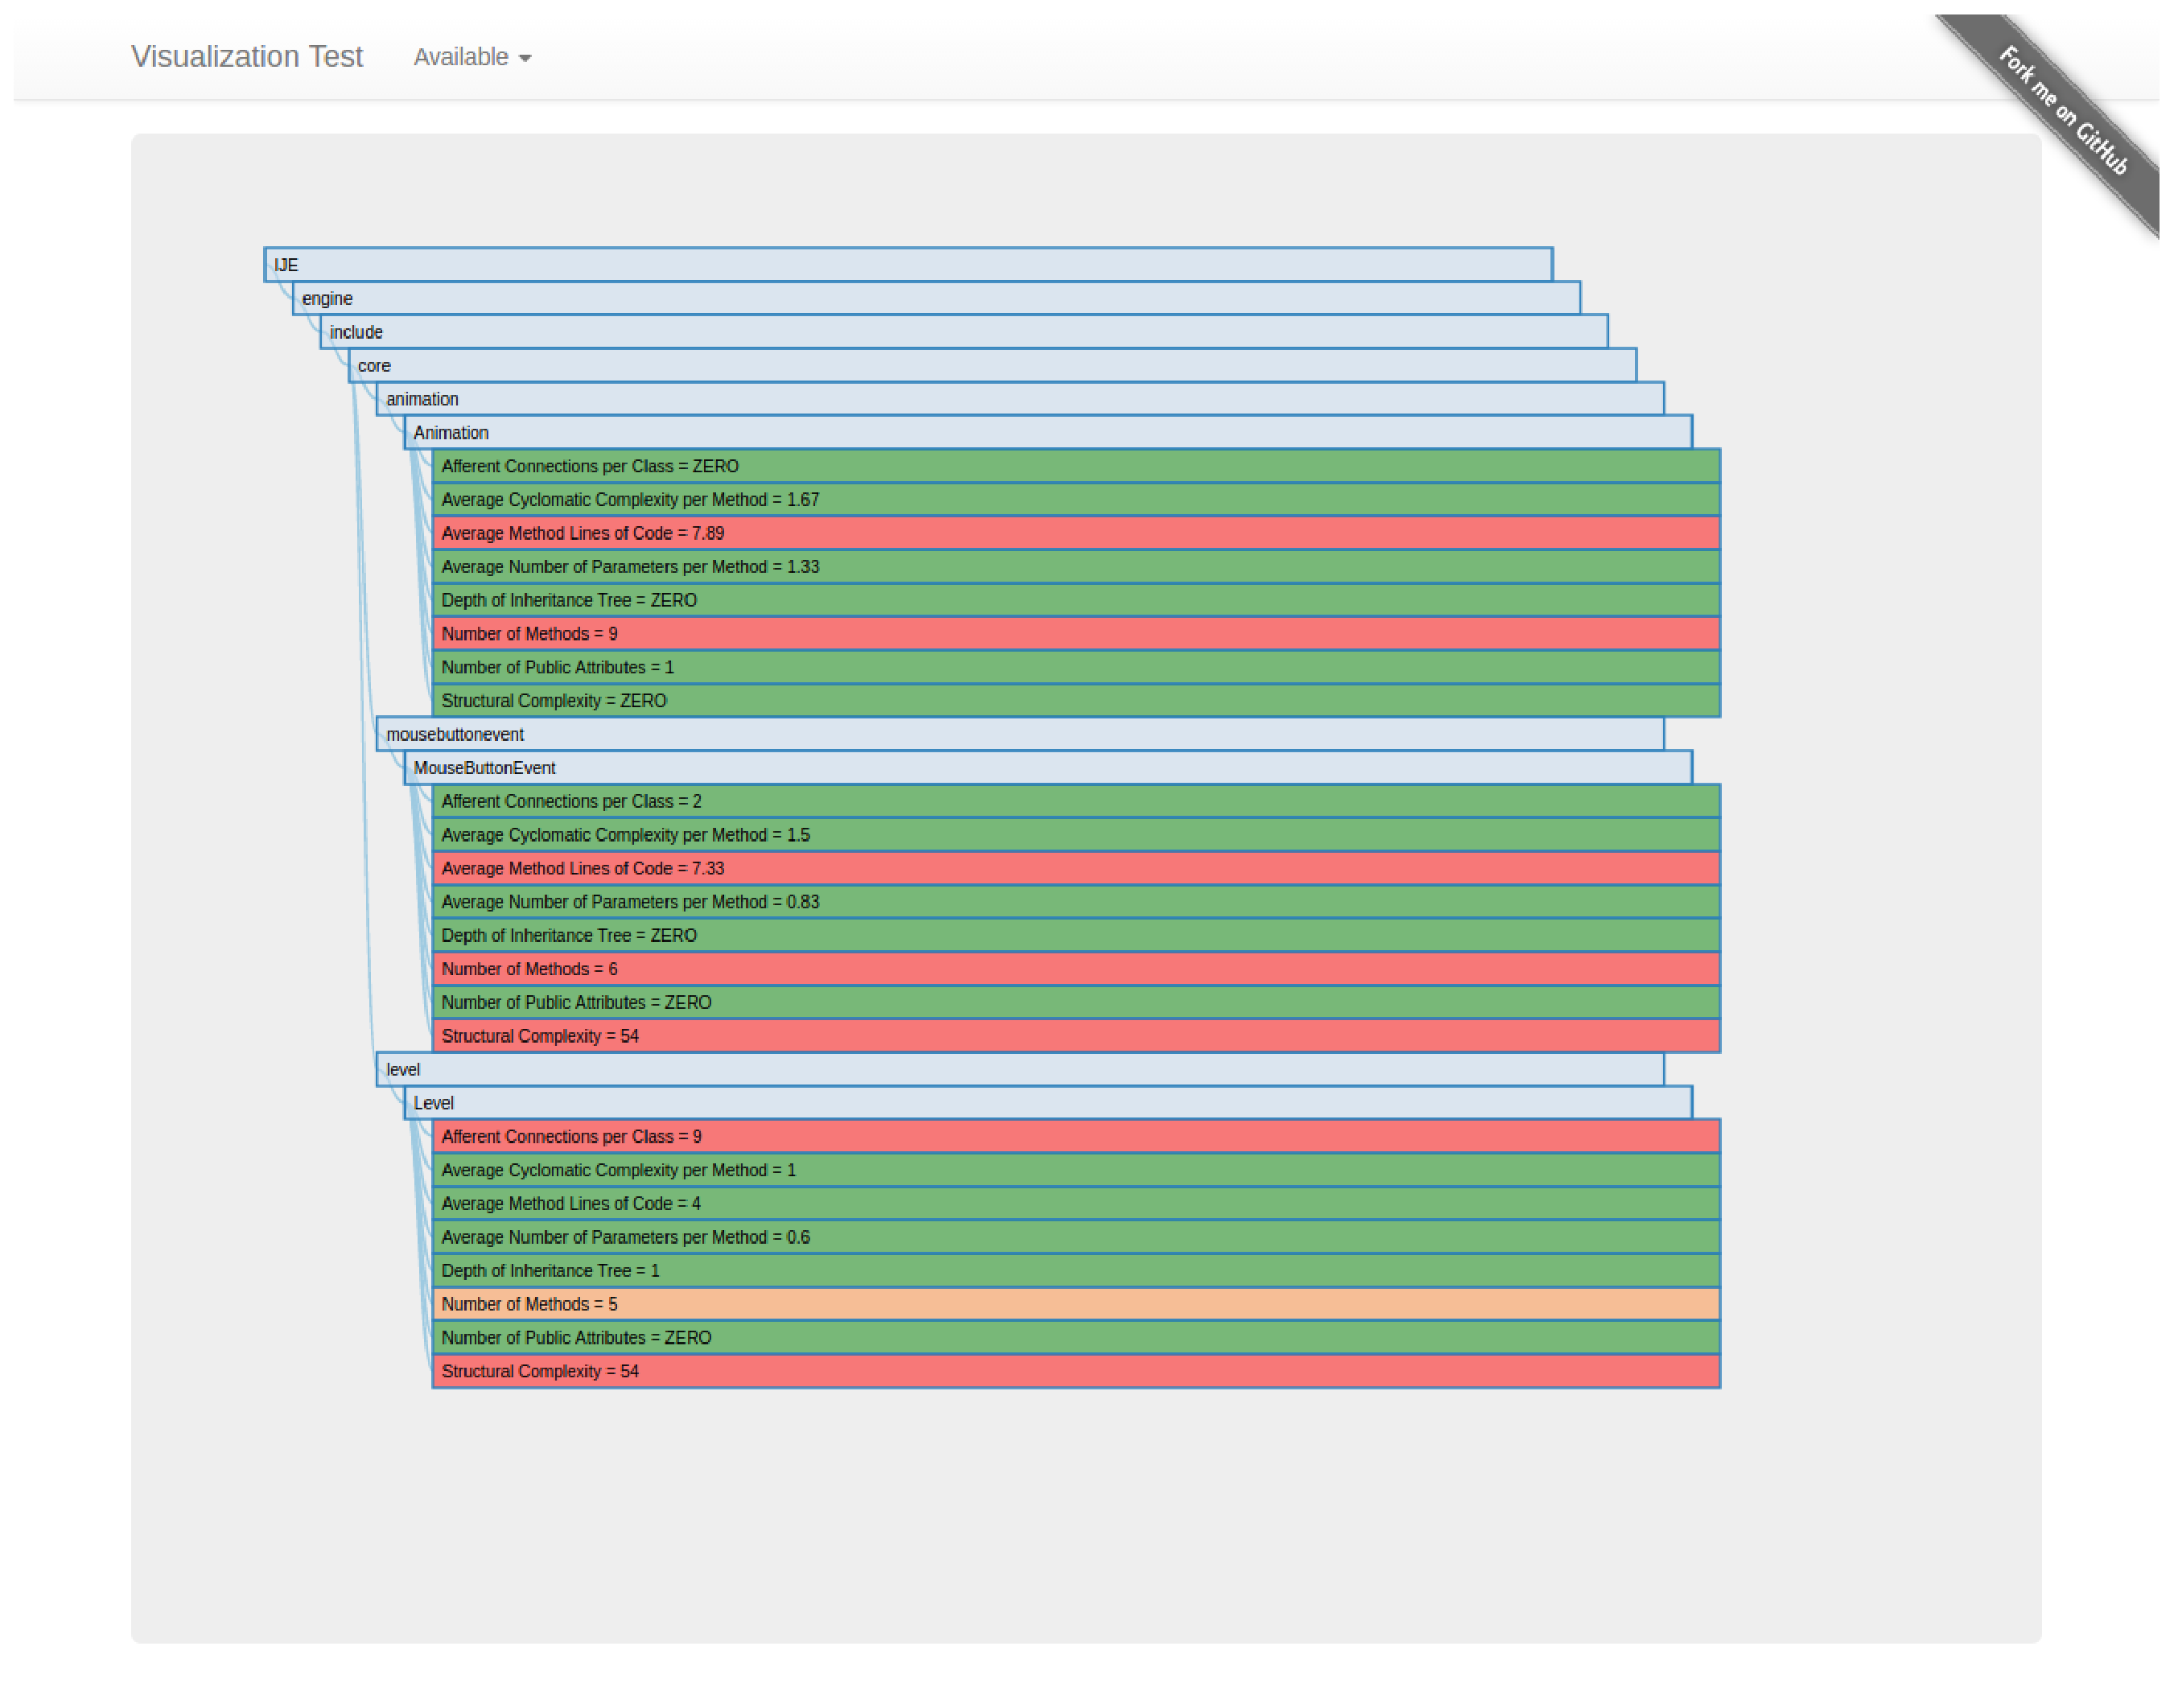
\includegraphics[keepaspectratio=true,scale=0.35]
    {figuras/node_link_tree_with_interaction.eps}
  \caption{Collapsible Indented Tree por Lars Kotthoff (adaptado)}
  \label{fig:node_link_tree_with_interaction}
\end{figure}

A segunda adaptação foi baseada no trabalho de Michael Bostock, \textit{Node
Link Tree, Radial Reingold – Tilford Tree}
\footnote{\url{http://bl.ocks.org/tpreusse/2bc99d74a461b8c0acb1}}. E a terceira
é adaptada de uma das visualizações criadas por Lars
Kotthoff\footnote{\url{http://bl.ocks.org/larskotthoff/7022289}}.

Para a exibição destas adaptações, foi realizado a construção de uma aplicação
Rails simplificada, apenas com o carregamento de páginas estáticas e hospedada
na plataforma Heroku. Pode ser acessada através do domínio
\href{https://visualizationtest.herokuapp.com/}{visualizationtest.herokuapp.com}.


Com o propósito de ser um teste de visualização de software, esta exibição foi
submetida à avaliação de estudantes e pessoas envolvidas com a Engenharia de
Software, perguntando:

\begin{itemize}
  \item[] \textit{Qual das visualizações você considera melhor para a
	interpretação das métricas?}
		\begin{itemize}
			\item {Random Radar Chart by Thomas Preusse (adapted)}
			\item {Node Link Tree by Mike Bostock (adapted)}
			\item {Node Link With Interation by Lars Kotthoff (adapted)}
		\end{itemize}
  \item[] \textit{Qual delas foi mais claro identificar os
	pontos/classes/métricas críticos e que merecem atenção?}
		\begin{itemize}
			\item {Random Radar Chart by Thomas Preusse (adapted)}
			\item {Node Link Tree by Mike Bostock (adapted)}
			\item {Node Link With Interation by Lars Kotthoff (adapted)}
		\end{itemize}
\end{itemize}

As Figuras \ref{fig:radar}, \ref{fig:node_link_tree} e
\ref{fig:node_link_tree_with_interaction} mostram estas adaptações disponíveis
na pequena aplicação Rails.
%
Com um total de 18 participantes, aproximadamente 60\% escolheu a visualização
feita por Lars Kotthoff (Node Link with Interaction - Collapsible Indented
Tree) como a melhor para interpretação das métricas e também para identificar
com mais claridade os pontos críticos. Os resultados completos estão no Apêndice
\ref{chap:apendiceA}.

Em suma, a proposta inicial de aplicação de técnicas de VS foi revogado ao
longo do desenvolvimento deste trabalho. Porém, os resultados propostos neste
experimento podem ser um passo inicial nesta direção.
